\documentclass[12pt]{article} % JASA requires 12 pt font for manuscripts
%\usepackage{JASA_manu}        % For JASA manuscript formatting

% for citations
\usepackage[authoryear]{natbib} % natbib required for JASA
\usepackage[colorlinks=true, citecolor=blue, linkcolor=blue]{hyperref}
\newcommand{\citetapos}[1]{\citeauthor{#1}{\textcolor{blue}{'s}} }

%\definecolor{Blue}{rgb}{0,0,0.5}

\usepackage{amsthm}

% for figures
\usepackage{graphicx}
\usepackage{caption}
\usepackage{subfig}
\captionsetup[subfloat]{font=normalsize}
%\usepackage{subcaption}
\graphicspath{{figures/}}
\newcommand{\hh}[1]{{\color{orange} #1}}
\newcommand{\al}[1]{{\color{red} #1}}

% color in tables
\usepackage{color}
\usepackage{colorbl}

% help with editing and coauthoring
\usepackage{todonotes}

% title formatting
\usepackage[compact,small]{titlesec} 
% page formatting
\usepackage[margin = 1in]{geometry}
\usepackage[parfill]{parskip}

% line spacing
\usepackage{setspace}
\doublespace

% For math typsetting
\usepackage{bm}
\usepackage{amstext}
\usepackage{amssymb}
\usepackage{amsmath}
\usepackage{amsfonts}
\usepackage{multirow}
\usepackage{lipsum}

\newtheorem{proposition}{Proposition}
\newtheorem{theorem}{Theorem}
\newtheorem{definition}{Definition}
\newtheorem{algorithm}[theorem]{Algorithm}

% A few commands to make typing less tedious
\newcommand{\inv}{\ensuremath{^{-1}}}
\newcommand{\ginv}{\ensuremath{^{-}}}
\newcommand{\trans}{\ensuremath{^\prime}}
\newcommand{\E}{\ensuremath{\mathrm{E}}}
\newcommand{\var}{\ensuremath{\mathrm{Var}}}
\newcommand{\cov}{\ensuremath{\mathrm{Cov}}}
\DeclareMathOperator{\tr}{Trace}
\DeclareMathOperator{\rank}{rank}
\DeclareMathOperator*{\argmin}{arg\,min}

\title{Are you Normal? The Problem of Confounded Residual Structures in Hierarchical Linear Models}
\author{
	Adam Loy and Heike Hofmann\\
	Department of Statistics,
	Iowa State University
}

\begin{document}
\maketitle

%----------------------------------------------------------------------------------
% Abstract

\begin{abstract}
We encounter hierarchical data structures in a wide range of applications. Regular linear models are extended by random effects to address correlation between observations in the same group. Inference for random effects is sensitive to  distributional mis-specifications of the model, making checks for (distributional) assumptions particularly important.  The investigation of residual structures is complicated by the presence of  different levels and corresponding  dependencies. Ignoring these dependencies leads to  erroneous conclusions using our familiar tools, such as Q-Q plots or normal tests. We first show the extent of the problem, then we introduce the {\it fraction of confounding} as a measure of the level of confounding in a model and finally introduce minimally confounded residuals as a solution to assessing distributional model assumptions.
\end{abstract}
{\bf Keywords:} Diagnostic, Multilevel model, Q-Q plot, Random effects distribution

%----------------------------------------------------------------------------------

%----------------------------------------------------------------------------------
\section{Introduction}\label{sec:intro}
%----------------------------------------------------------------------------------
There is a wide range of application areas---from the biological and physical sciences to the social sciences---in which we encounter nested  data.
Whether it is quality control in a manufacturing process that involves the monitoring of a set of components over  time  or students' performances in different schools across the country, analysts have to account for  the correlation between observations in the same group.  Hierarchical linear models \al{(i.e., multilevel models, linear mixed effects models)} allow us to do exactly that---but they also require us to make distributional assumptions on both the error terms and the random effects. These assumptions must hold to ensure the validity of the model \hh{and all of its resulting conclusions.} 
Inference for the fixed effects in linear mixed models is fairly robust against model mis-specification \citep{Butler:1992tx, Verbeke:1997tf}. This is different for random effects: they are sensitive to  distributional mis-specifications and  therefore have to be checked carefully, especially when they are central to the inferential goals, such as in the construction of a prediction interval for an unobserved group.

Quantile-quantile (Q-Q) plots \citep{Wilk:1968} are our main graphical tool for evaluating a specific distributional assumption. For that, we plot the empirical distribution against the expected quantiles from the assumed distribution. In hierarchical linear models the investigation of residual structures is complicated by the presence of  different levels. 
The nested structure of the data is reflected in the residual structure, and just as there is dependence between different levels in the data, we can expect dependencies between different levels in the residual structure. Q-Q plots, {in their} weighted \citep{Dempster:1985tr, Lange:1989uu} or unweighted {form}, do not account for this, which can lead us to erroneous conclusions in evaluating normality based on the plots. \hh{Unfortunately, the same is true for any other standard test. } % (or any other \al{standard} test).

% however, these plots, weighted or unweighted, do not account for the relationship between the predicted random effects and error terms and result in inflated type I error rates. 

%From a graphical perspective the assessment of the assumptions made on the random effects has focused on plotting the empirical distribution of the predicted random effects in quantile plots 

In this paper, we address the problem of distributional assessment due to confounding in residual structures. 
First, we illustrate the inadequacy of existing methods  based on the predicted residuals. 
We then introduce  the concept of \al{rotated} residuals for the random effects and present a general method to obtain \al{rotated} residuals for residuals at all levels of the model. We demonstrate how this enables an appropriate (graphical) assessment  of distributional assumptions.
\todo[inline]{Return to this paragraph after more writing...}


\section{Motivating example}\label{sec:ex}
%To motivate our discussion
To illustrate the effect of confounding between different levels of residuals, we consider the data set discussed by
 \cite{Gelman:2006ue}. This data set consists of a stratified random sample of 919 owner-occupied homes nested within 85 counties in Minnesota, for which the authors suggested a hierarchical model of the form
%
\begin{equation}\label{eq:radon}
  \log(y_{ij}) = \beta_0 + \beta_1 x_{1ij} + \beta_2 x_{2i} + b_{0i} + b_{1i} x_{1ij}  + \varepsilon_{ij}
\end{equation}
%
where   $\log(y_{ij})$ denotes the  radon measurement (in log $pCi/L$, i.e log picoCurie per litre) for house~$j$ ($1 \le j \le n_i, 1 \le i \le 85$) within county~$i$,
 $x_{1ij}$ is a binary variable describing the level at which the measurement was taken (0 for the basement and 1 for a higher level) and $x_{2i}$ denotes the average soil uranium content for  county~$i$. 
 Further, we assume i.i.d. normal errors $\varepsilon_{ij} \sim \mathcal{N} (0,\ \sigma^2_{\varepsilon})$  and $\bm{b}_i \sim \mathcal{N}(\bm{0},\ \bm{D})$, where $\bm{D}$ allows for correlation between $b_{0i}$ and $b_{1i}$. We also assume independence between random effects and error \al{terms}. 


A map of counties in Minnesota is given in figure \ref{fig:map}. The color shading represents average radon activity in a county. For two counties no data is available. Generally, more southern locations exhibit higher  levels of Radon activity. Figure \ref{fig:tc} focuses on the two counties of Hennepin (home to Minneapolis) and Winona (home to the city of the same name). Radon levels are plotted by floor level. Radon levels are usually the highest at the basement level of a house. 
%
\begin{figure}[htb]
\centering
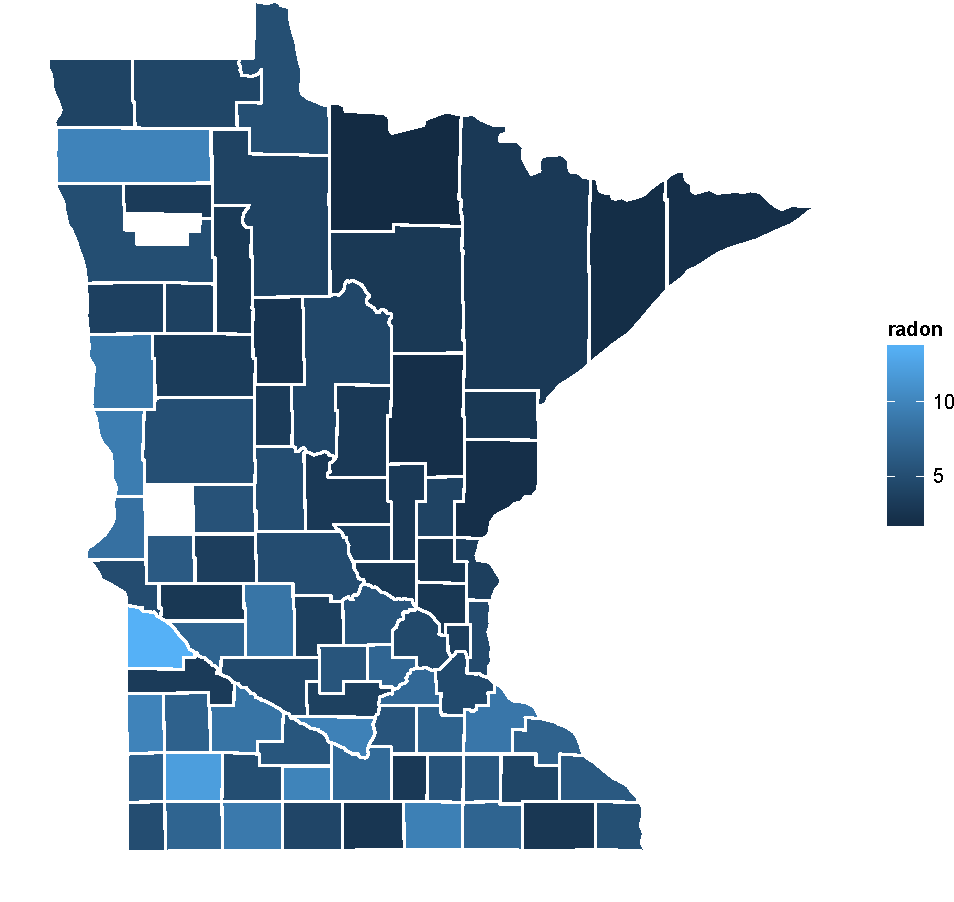
\includegraphics[width=0.5\linewidth]{figures/map-cropped.pdf}
\caption{\label{fig:map} Map of the counties in Minnesota. The color shading represents average Radon activity.}
\end{figure}
%
\begin{figure}[htb]
\centering
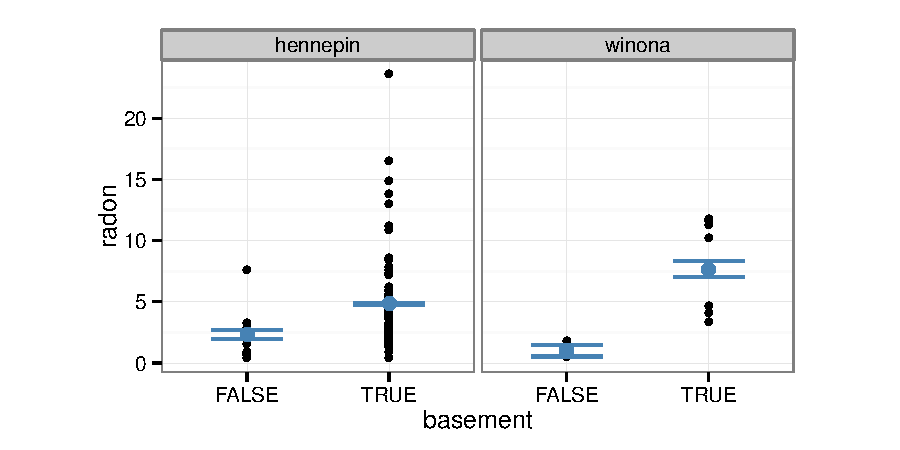
\includegraphics[width=0.7\linewidth]{figures/radon-twocounties.pdf}
\caption{\label{fig:tc} Activity of radon levels for Hennepin and Winona counties at basement levels and higher. 95\% confidence intervals for the sample mean are given by the error bars. Radon levels at the basement level are usually higher.}
\end{figure}
%
The within-county sample sizes, $n_i$, are extremely unbalanced, ranging from one house to 116 houses, with 50\% of the counties having between three and ten houses. Such unbalanced designs are common in applications, and result in a high degree of pooling \al{(shrinkage)} for the predicted county-level random effects. \hh{XXX why the parenthesis? - This might need another sentence, because pooling is what leads to shrinkage, which in turn leads to residual dependencies on different levels.}
\al{XXX I use the terms pooling and shrinkage to refer to the same concept as discussed in \cite{Gelman:2006ue}, that is why I put shrinkage in parentheses, so that those who are more familiar with shrinkage see the point I am trying to make. Perhaps is should be `(i.e., shrinkage)' instead? I can still think about adding some clarification id this is still confusing.}
 % \citep[see][figure 3]{Gelman:2006ue}. 
This leads to dependence between  predicted random effects and  error terms (cf. eqns. \ref{eq:resid1} and \ref{eq:resid2}), which in turn can lead us to draw erroneous conclusions for corresponding residual quantities.


\begin{figure}[!h]
	\centering
	  \subfloat[Predicted error terms]{
		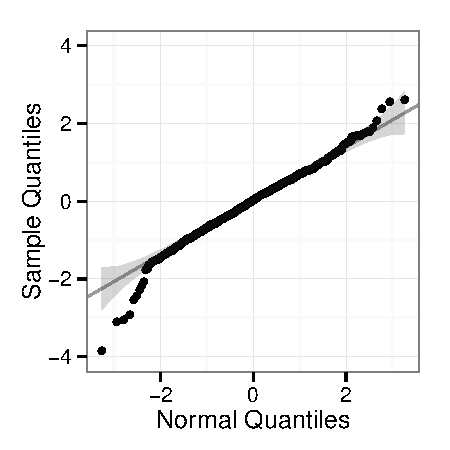
\includegraphics[width=0.33\linewidth]{raw-lev1-qq.pdf}
	   }
	  \subfloat[Random intercepts]{
		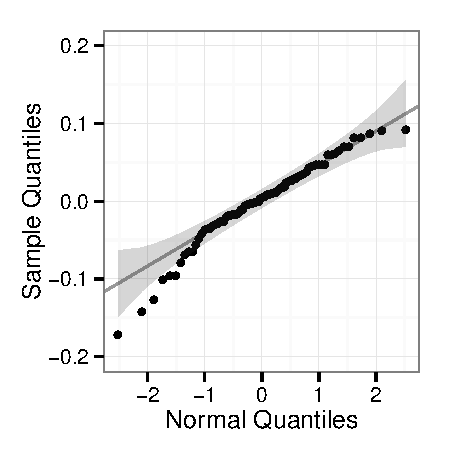
\includegraphics[width=0.33\linewidth]{raw-intercept-qq.pdf}
		}
%	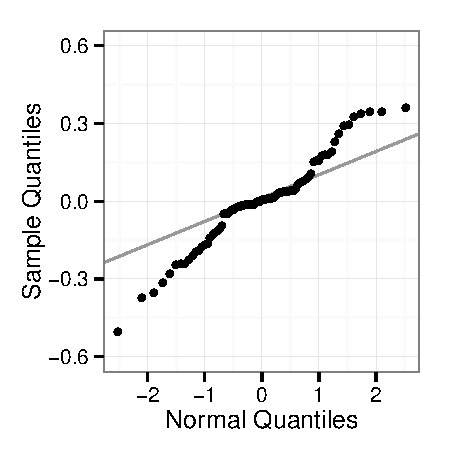
\includegraphics[width=0.32\textwidth]{raw-slope-qq.pdf}
	\caption{\label{fig:qqplots1} Q-Q plots of predict\al{ed residuals} at different levels %, and random slopes (right) 
	for model~\eqref{eq:radon}. \hh{Both plots suggest a deviation of residuals from a normal distribution.} Note that random slopes (see figure~\ref{fig:lineup}) exhibited the largest deviation from normality. }
\end{figure}

\begin{figure}[htb]
	\centering
	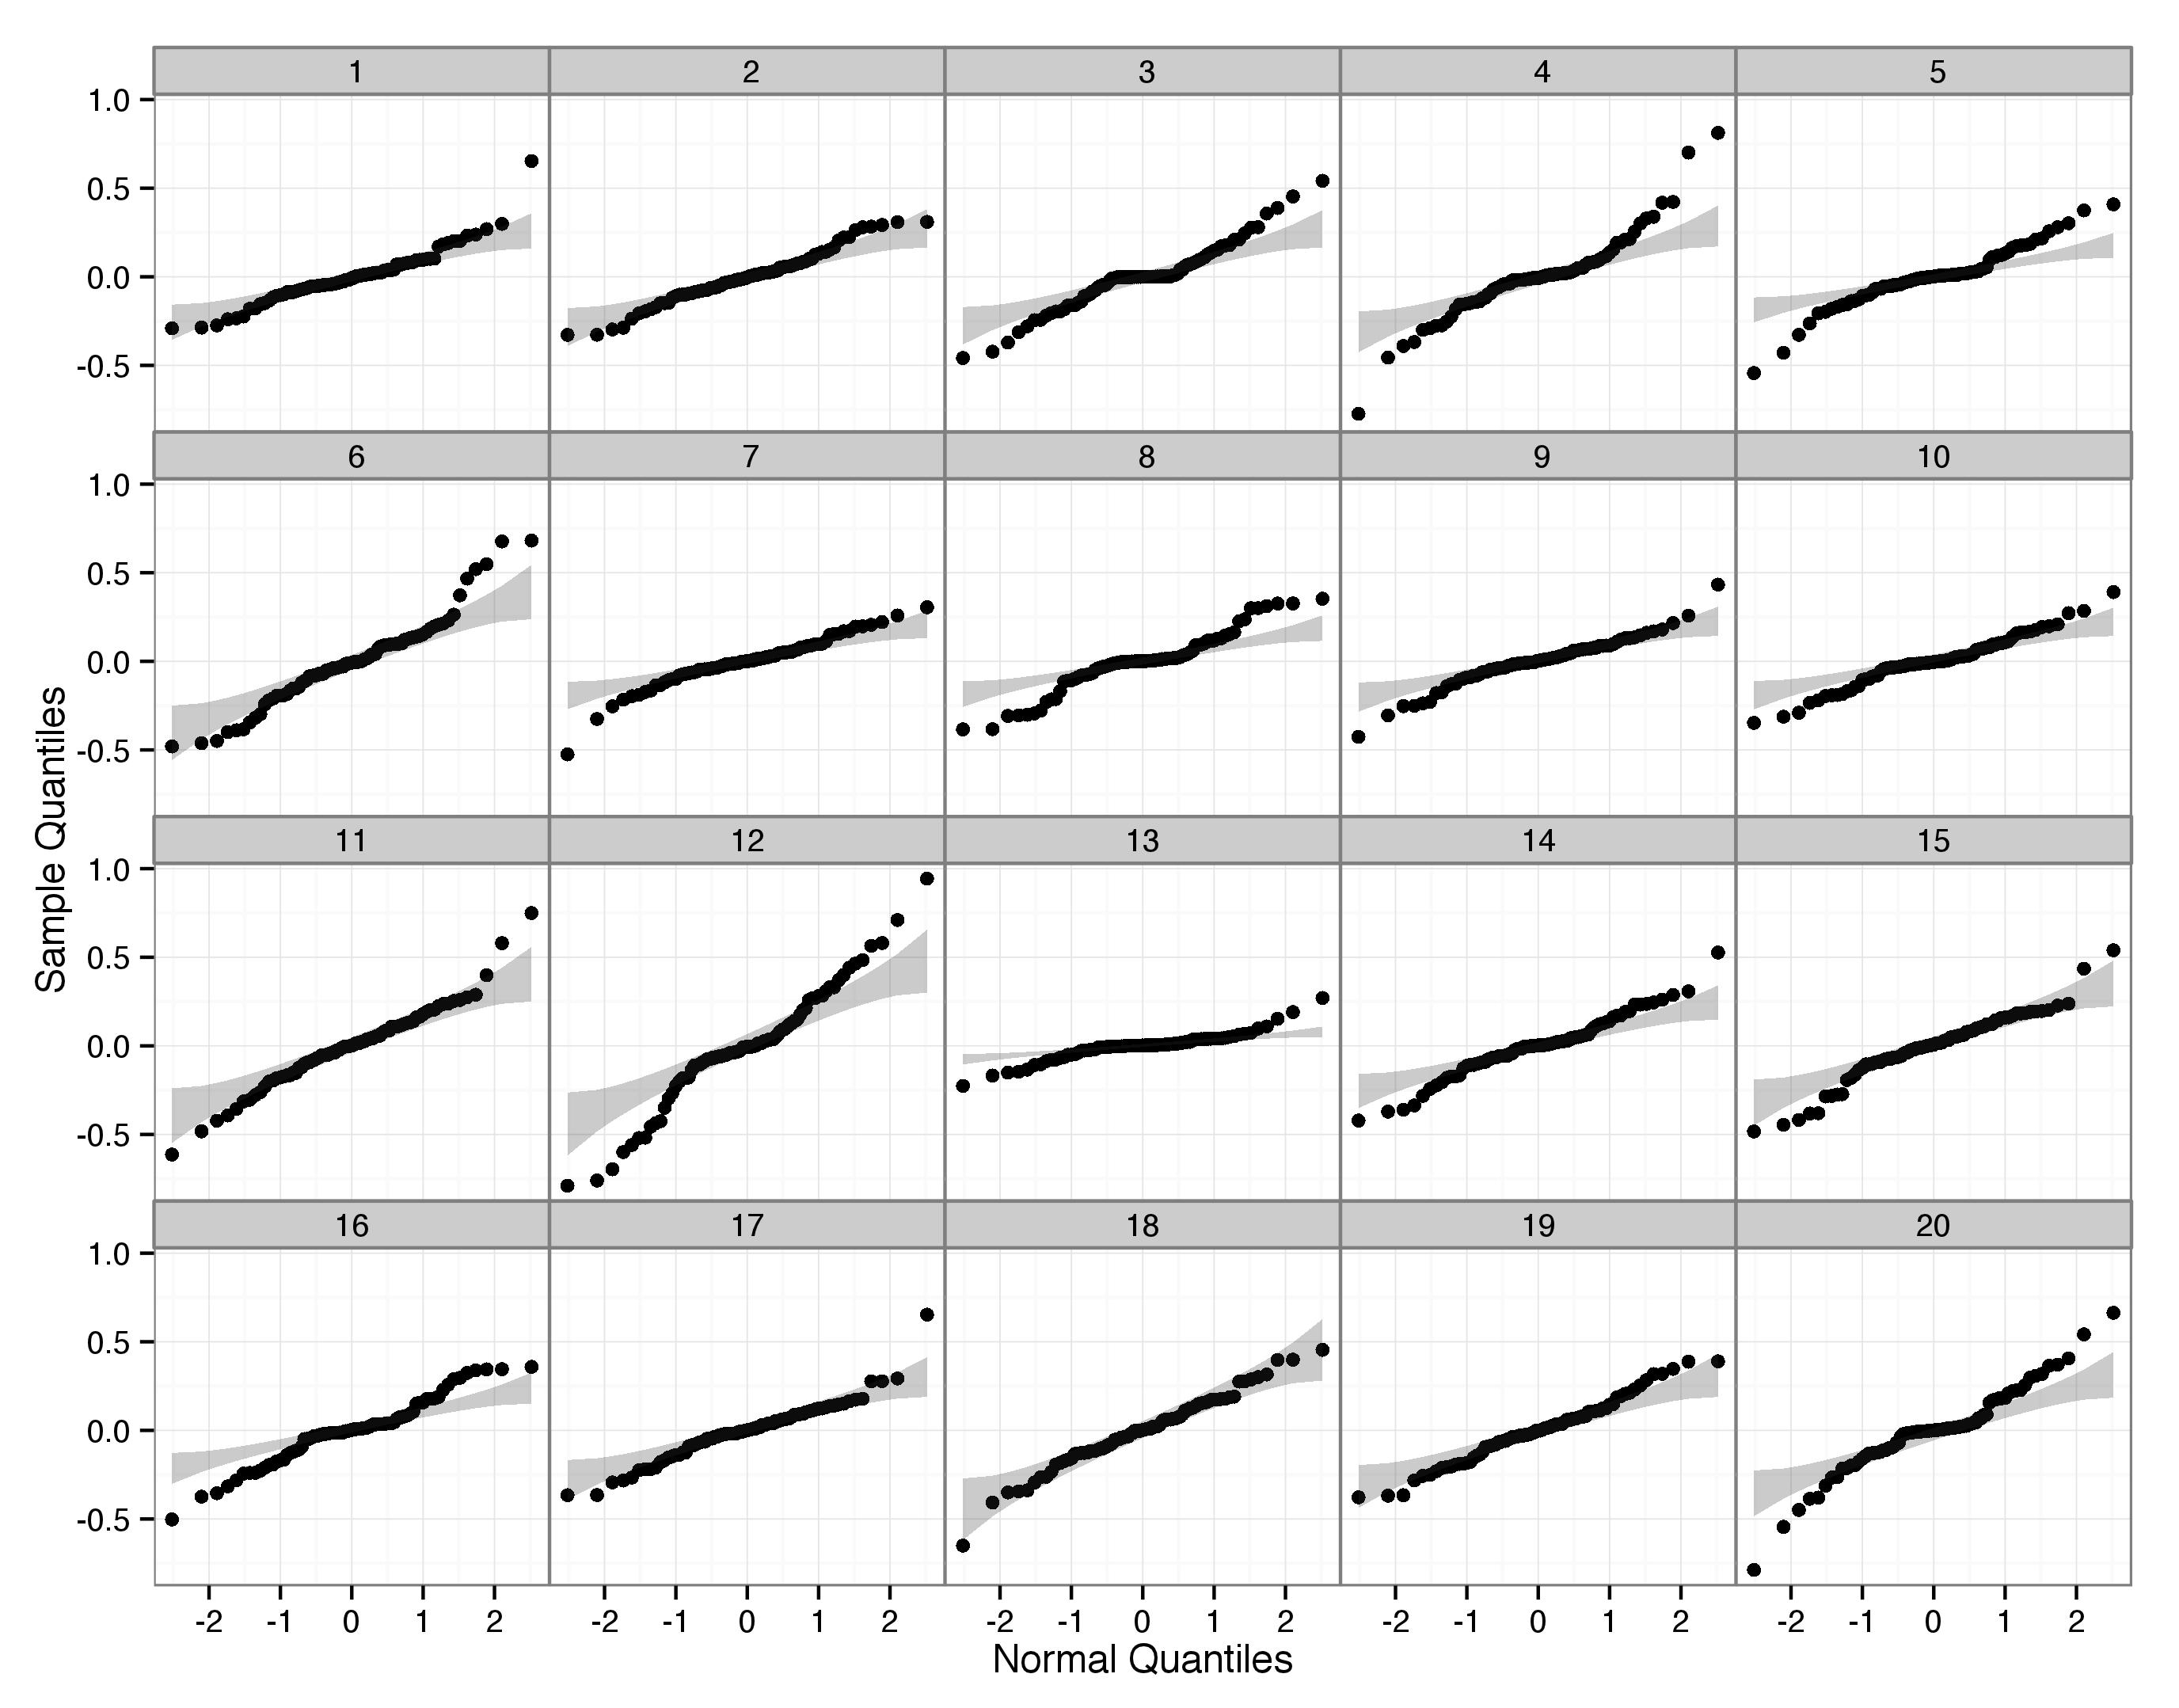
\includegraphics[width=0.9\textwidth]{test.jpeg}%lineup-rslope.pdf}
	\caption{\label{fig:lineup} Lineup of normal Q-Q plots for the random slope term in model~\eqref{eq:radon}. The 19 null plots were obtained by simulation from the model. Can you identify the observed Q-Q plot? }
\end{figure}


In this example, Q-Q plots (Figure~\ref{fig:qqplots1}) for the residuals show that normality 
seems to be violated for the error terms and both random effects. But is this cause for concern?
\al{As} there is little pooling at the observation level \al{(level 1)} we expect the distributional assessment of the error terms to be reliable, but  the high degree of pooling  for the random effects  casts doubt on the reliability of their Q-Q plots. 
 We find our doubts increasing in a simulation-based assessment of distributions for residuals and random effects.

Figure~\ref{fig:lineup} shows a lineup \citep{buja:2009} of 20 Q-Q plots for the predicted random slope. The Q-Q plot of the observed random slopes is placed among 19 decoy plots of parametric bootstrap samples based on model~\eqref{eq:radon} satisfying the normal distribution assumptions. The simulation parameters were set to the maximum likelihood estimates of model~\eqref{eq:radon}.
The observed Q-Q plot (panel $12+2^2$) is virtually indistinguishable from the field of null plots. This suggests that the predicted random slopes  from the data do not deviate significantly from model~\eqref{eq:radon}. 
%A lineup of the random intercepts revealed the same finding and was omitted for brevity. 
Note that in practice we must blind ourselves from the true plot for proper use of lineups. In order to not violate this, we did not show the Q-Q plot of random slopes earlier.
%
%application of the Anderson-Darling test results in the rejection of the null hypothesis of normality at the .05 significance level for the error terms and both random effects. As there is little pooling at the observation level we would expect the distributional assessment of the error terms to be reliable, but this is not the case with the random effects. 
%
%To further explore the distributional assumptions made on the random effects we create lineups \citep{buja:2009} of quantile plots were created by randomly inserting the true quantile plot for each term into a field of 19 plots generated under the null hypothesis of normality. A lineup for the random slopes is presented in Figure~\ref{fig:lineup}. The observed quantile plot (panel 16) is indistinguishable from the field of null plots, indicating that these predicted random slopes do not deviate from what would be expected under model~\eqref{eq:radon}, contradicting the results of the AD test. 

What becomes apparent from the lineup, is that, astonishingly, {\it none} of the null plots conforms to normality. Further investigation  reveals  that a  proportion far above the nominal 0.05 of distributions of random intercepts also fail the normality tests.


%Further evidence of the impact of this dependence is evident from a small scale simulation study. We used the design of the radon study to simulate 5000 data sets under model~\eqref{eq:radon} satisfying the assumptions discussed above. The simulation parameters were set to the maximum likelihood estimates of model~\eqref{eq:radon}. 
%%: $\widehat{\beta_0} = 1.46$, $\widehat{\beta_1} = -0.64$, $\widehat{\beta_2} = 0.77$, $\widehat{\sigma}_{\varepsilon} = 0.75$, $\widehat{\sigma}_{b_0} = 0.12$, $\widehat{\sigma}_{b_1} = 0.35$, and $\widehat{\rho} = 0.26$. 


Table~\ref{tab:edf} shows results from 1000 parametric bootstrap samples of model~\eqref{eq:radon} assuming normal random effects and level-1 residuals generated as normal, heavy tailed ($\varepsilon_{ij}^* \overset{iid}{\sim} (\sigma_{\varepsilon} / \sqrt{3})\, t_3$), and skewed ($\varepsilon_{ij}^* \overset{iid}{\sim} \sigma_{\varepsilon} \, \{ \text{Exp}(1) - 1 \}$).
For each simulated data set, we evaluated the assumption of normality for both the level-1 and -2 residuals using the Anderson-Darling (AD), Cram{\'e}r von Mises (CVM) and  Kolmogorov-Smirnov (KS) tests for normality.  
%Table~\ref{tab:edf} shows the proportions of the tests of the empirical distribution function rejecting the null hypothesis of normality at the .05 significance level. 
The type I error rates are hugely inflated both random effects, making an assessment of normality based on the empirical distribution impossible. Use of standardized random effects and \citetapos{Lange:1989uu} weighted Q-Q plot reduce the type I errors to the nominal level when the level-1 residuals are normal, but the type I errors remain inflated for non-normal level-1 residuals. Similarly, when the random effects are not normal, simulations (not shown) revealed that the tests were unable to reject the null hypothesis of normality when the level-1 residuals were normal. \al{From the above we see that distributional assessment of the predicted random effects is confounded by the distribution of the level-1 residuals.}
%The inflated type I error rates for the random effects indicate that the empirical distribution of the random effects cannot be used to assess the assumption of normality. 
In this example we are able to use the empirical distribution to assess normality of  level-1 residuals  as  pooling is minimal at this level. In situations with higher levels of pooling, this may not be the case.

\begin{table}[t]
\centering
\caption{\label{tab:edf} Proportions of tests rejecting the null hypothesis of normality of the predicted random intercept and slope at the nominal .05 significance level when the error terms are normal, heavy tailed, and skewed. The type I error rates are hugely inflated under each setting. \vspace{.5em}}
\subfloat[Random intercept]{
	\begin{tabular}{l rrr} \hline
	& \multicolumn{3}{c}{Test} \\ \cline{2-4}
	  	&     AD & CVM  & KS \\ \hline
	Normal       	   &	 0.655 & 0.612 & 0.471  \\ 
	Heavy tailed 	   & 0.910 & 0.903 & 0.802  \\ 
	Skewed       	   & 0.847 & 0.821 & 0.710  \\  
	\hline
	\end{tabular}
}
\qquad
\subfloat[Random slope]{
	\begin{tabular}{l rrr} \hline
	& \multicolumn{3}{c}{Test} \\ \cline{2-4}
	  	&     AD & CVM  & KS \\ \hline
	Normal       	  & 0.739 & 0.712 & 0.591  \\ 
	Heavy tailed 	  &	0.939 & 0.938 & 0.8691  \\ 
	Skewed       	  &	0.888 & 0.866 & 0.792  \\  
	\hline
	\end{tabular}
}


%\subfloat[Standardized Random intercept]{
%	\begin{tabular}{l rrr} \hline
%	& \multicolumn{3}{c}{Test} \\ \cline{2-4}
%	  	&     AD & CVM  & KS \\ \hline
%	Normal       	   &	 0.048 &	 0.045 &	 0.046  \\ 
%	Heavy tailed 	   & 0.349 & 0.325 & 0.256  \\ 
%	Skewed       	   & 0.520 & 0.487 & 0.399  \\  
%	\hline
%	\end{tabular}
%}
%\qquad
%\subfloat[Standardized Random slope]{
%	\begin{tabular}{l rrr} \hline
%	& \multicolumn{3}{c}{Test} \\ \cline{2-4}
%	  	&     AD & CVM  & KS \\ \hline
%	Normal       	  & 0.039 &	0.041 &	0.048  \\ 
%	Heavy tailed 	  &	0.434 & 0.403 & 0.320  \\ 
%	Skewed       	  &	0.540 & 0.504 & 0.422  \\  
%	\hline
%	\end{tabular}
%}

\end{table}


%\begin{table}[!h]
%\caption{\label{tab:edf} Proportions of tests rejecting the null hypothesis of normality of the predicted error terms and random effects at the nominal .05 significance level. \hh{didn't we want to keep the  background for power? - it should be consistent throughout the paper} Type I error rates are hugely inflated. \vspace{.5em}
%}
%\begin{center}
%\begin{tabular}{l rrr} \hline
%& \multicolumn{3}{c}{Test} \\ \cline{2-4}
% Residual &  AD & CVM & KS \\ \hline
%Error term			 & 0.06 & 0.06 & 0.05\\
%\rowcolor{gray!20} Random intercept 	& 0.48 & 0.46 & 0.35\\
%\rowcolor{gray!20} Random slope 		& 0.75 & 0.75 & 0.68\\
%   \hline
%\end{tabular}
%\end{center}
%\end{table}


In the remainder of this paper we investigate the root of concern that leads to the distributional deviations, and derive residuals that address the issues introduced by pooling, allowing again for a familiar graphical assessment of these distributions.

%----------------------------------------------------------------------------------
\section{Hierarchical linear models and residuals}\label{sec:resid}
%----------------------------------------------------------------------------------
The general stacked representation of the hierarchical linear model is given by
%
\begin{eqnarray}\label{eq:hlm}
 && \bm{y} = \bm{X \beta} + \bm{Z b} + \bm{\varepsilon}, \\ \nonumber
 && \E \begin{bmatrix} \bm{b} \\ \bm{\varepsilon} \end{bmatrix} = \bm{0}, 
 \ \cov \begin{bmatrix} \bm{b} \\ \bm{\varepsilon} \end{bmatrix} = 
  	\begin{bmatrix} \bm{D} & \bm{0}\\ \bm{0} & \bm{R} \end{bmatrix}
\end{eqnarray}
%
where $\bm{y}$ is an $n \times 1$ vector of observed responses, $\bm{X}$ ($n \times p$) and $\bm{Z}$ ($n \times q$) are design matrices, $\bm{\beta}$ is a $p \times 1$ vector of unknown fixed effects, $\bm{b}$ is a $q \times 1$ vector of unobserved random effects, $\bm{\varepsilon}$ is an $n \times 1$ vector of unobserved errors, and $\bm{R}$ and $\bm{D}$ are positive definite covariance matrices.

  %Additionally, it is often assumed that $\bm{\varepsilon}$ and $\bm{b}$ are normally distributed. 
Using this specification, the predicted error terms and random effects are given by 
%
\begin{align}
\widehat{\bm{\varepsilon}} &= \bm{RPy} = \bm{RPZb} + \bm{RP \varepsilon} \label{eq:resid1}\\
\widehat{\bm{b}} &= \bm{DZ}\trans \bm{Py} = \bm{DZ}\trans \bm{PZb} + \bm{DZ}\trans \bm{P \varepsilon} \label{eq:resid2}
\end{align}
%
where $\bm{P} = \bm{V}\inv( \bm{I} - \bm{X} (\bm{X}\trans \bm{V}\inv \bm{X})\inv \bm{X}\trans \bm{V}\inv)$. This  set of equations %\eqref{eq:resid1} and \eqref{eq:resid2} 
reveals the inherent dependence between the residuals.
Additionally, it is easily seen that both \eqref{eq:resid1} and \eqref{eq:resid2} lead to the analysis of correlated and potentially heteroscedastic disturbances as $\var(\widehat{\bm{\varepsilon}}) = \bm{RPR}$ and $\var(\widehat{\bm{b}}) = \bm{DZ}\trans \bm{PZD}$.
\al{
The use of standardized residuals can correct the latter issue, but does not address the fact that the residuals are interrelated. While problems may be expected at both levels of the model based on \eqref{eq:resid1} and \eqref{eq:resid2}, we have found that the interpretation of Q-Q plots of the standardized predicted error terms
%
\[
\bm{z}_{\varepsilon} =  \text{diag} \left(\bm{RPR} \right)^{-1/2} \widehat{\bm{\varepsilon}}
\]
%
is unaffected by this interrelationship; however, this is not the case with the random effects.  When the degree of pooling is high---as it is in the above radon example, and often is in practice---interpretation of the predicted random effects cannot be separated from the distribution of the error terms. Detailed simulation results \hh{documenting} the utility of  these residuals are available in the supplementary material.
}


%----------------------------------------------------------------------------------
\section{Rotating the random effects}\label{sec:rotate}
%----------------------------------------------------------------------------------

To combat \al{the confounded nature of the predicted random effects}, we derive a reduced set of minimally confounded residuals that are standardized, uncorrelated, and homoscedastic. \al{We focus our discussion (and notation) on a two-level model with a single random effect in this section for ease of explanation, and we describe how to extend this method at the end of this section.} \cite{HildenMinton:1995wh} presents the derivation of a similar set of minimally confounded residuals for the error terms, but does not address the random effects which are the focus of this paper. 

First, we define the \emph{fraction of confounding} for the random effects, which is minimized in the result below. This definition generalizes the fraction of confounding proposed by \cite{HildenMinton:1995wh}. \\

%\begin{definition}[Fraction of confounding]\label{def:fc1}
%For the $i$th element of the target residual vector, $\widehat{\bm{e}}$, the fraction of confounding is given by
%%
%\begin{equation}\label{eq:fc}
%	\text{FC}(\widehat{\bm{e}}_i) 
%	= \frac{\bm{v_i}\trans \var(\widehat{\bm{e}} | \bm{e}) \bm{v_i}}
%		{\bm{v_i}\trans \var(\widehat{\bm{e}}) \bm{v_i}}
%	= \frac{\bm{v_i}\trans \bm{A} \bm{v_i}}
%		{\bm{v_i}\trans \bm{B} \bm{v_i}}
%\end{equation}
%
%where $\bm{v_i}$ is the $i$th column of the identity matrix.
%%\todo[inline]{write this as a minimization problem}
%%This rotation is given by $\bm{M} = \bm{T_r \Lambda_r}^{-1/2} \bm{U}$ where $\bm{T_r \Lambda_r}^{-1/2}$ is the inverse square root of $\bm{B}$ found through the spectral decomposition of $\bm{B}$ and $\bm{U}$ are the eigenvectors of $(\bm{\Lambda_r}^{-1/2} \bm{T_r}\trans) \bm{A} (\bm{\Lambda_r}^{-1/2} \bm{T_r}\trans)\trans$.
%\end{definition}

%Definition~\ref{def:fc1} describes the confounding for each element in the target residual vector individually. An overall measure of the amount of confounding is given below.\\

%\begin{definition}\label{defc:fc2}
%For the target residual vector, $\widehat{\bm{e}}$, the fraction of confounding is given by
%%
%\begin{equation}\label{eq:fc2}
%FC(\widehat{\bm{e}}) = \mathrm{tr}( \var(\widehat{\bm{e}} | \bm{e} ) ) / \mathrm{tr}( \var(\widehat{\bm{e}}) ).
%\end{equation}
%\end{definition}

\begin{definition}[Fraction of confounding]
Let $\bm{A} = \var(\widehat{\bm{b}} | \bm{b} )$ and $\bm{B} = \var(\widehat{\bm{b}})$, which are positive semidefinite matrices by definition, then the fraction of confounding in $\widehat{\bm{b}}$ is given by
%
\begin{equation}\label{eq:fc2}
\text{FC}(\widehat{\bm{e}}) = \frac{1}{\ell} \tr\left( \bm{B}\ginv\bm{A} \right)
%\dfrac{1}{\ell} \displaystyle{\sum_i} \frac{\bm{v_i}\trans \bm{A} \bm{v_i}}
%		{\bm{v_i}\trans \bm{B} \bm{v_i}}.
\end{equation}
where $\ell$ is the length of vector $\widehat{\bm{b}}$.
\end{definition}
The fraction of confounding measures the contribution of the error terms  to the variance of the random effects. $\text{FC} \in [0,1]$, where 1 indicates predicted random effects contain no information in addition to that found in the error terms due to confounding, while 0 indicates no confounding. 


In order to correct residuals for the impact of confounding, we propose using a linear transformation of the random effects, $\bm{W}^{*\prime} \widehat{\bm{b}}$, that projects the random effects into $s$-dimensional space and satisfies
%find weights $\bm{w_i}$ to apply to each of the residual contributions that minimize $\tr\left( \bm{B}\ginv\bm{A} \right)$. This can be re-expressed as the following minimization problem:
%\[
%\bm{w}_{\ell-r} = \arg \min_{w \neq 0} \frac{\bm{w}\trans \bm{A} \bm{w}}
%		{\bm{w}\trans \bm{B} \bm{w}}.
%\]
\begin{equation}\label{eq:minimize}
\bm{W}^* = \argmin_{W \in \mathbb{R}^{\ell \times s} } 
\tr\left( \left(\bm{W\trans B W} \right)\inv \left(\bm{W\trans A W}\right) \right)
%\displaystyle{\sum_i} \frac{\bm{v_i}\trans \bm{W} \bm{A} \bm{W}\trans \bm{v_i}}
%		{\bm{v_i}\trans \bm{W} \bm{B} \bm{W}\trans \bm{v_i}}
\end{equation}
where $\ell$ is the length of vector $\bm{b}$. %and $r = \text{rank}(\bm{B})$. 
\al{This problem is solved using the generalized eigenvalue decomposition
\begin{equation}\label{eq:geigen}
	\bm{Aw}_k = \gamma_k \bm{Bw}_k
\end{equation}
where $\gamma_k$ and $\bm{w}_k$ are the $k$-th smallest eigenvalues and eigenvectors, respectively \citep{Fukunaga:1990}; thus, $\bm{W}^*$ consists of the eigenvectors associated with the $s$ smallest eigenvalues. Computationally, this problem can be solved by simultaneous diagonalization of $\bm{A}$ and $\bm{B}$. We outline this procedure below for reference and refer the reader to \cite{McDonald:1979ca} and \cite{deLeeuw:1982to} for additional details on simultaneous diagonalization of two positive semidefinite matrices.\\}

\begin{algorithm}[Simultaneous diagonalization]
Let $\bm{A}$ and $\bm{B}$ be two positive semidefinite matrices. The transformation that simultaneously diagonalizes both matrices can be found through the following procedure:
\begin{enumerate}
\item Find a transformation that whitens $\bm{B}$. Such a transformation is given by $\bm{T_r \Lambda_r}^{-1/2}$, where $\bm{T}_r$ and $\bm{\Lambda}_r$ are the first $r$ eigenvectors and eigenvalues of $\bm{B}$, where $r = \rank(\bm{B})$. 

\item Transform $\bm{A}$ and $\bm{B}$ to
\begin{align}
\bm{\Lambda_r}^{-1/2} \bm{T_r}\trans \bm{A T_r \Lambda_r}^{-1/2} &= \bm{A}^* \label{eq:astar} \\
\bm{\Lambda_r}^{-1/2} \bm{T_r}\trans \bm{B T_r \Lambda_r}^{-1/2} &= \bm{I}
\end{align}

\item Find an orthonormal transformation that diagonalizes $\bm{A}^*$. Such a transformation is given by the eigenvectors of $\bm{A}^*$, which we denote $\bm{U}$.
\end{enumerate}

Based on the above three steps, the transformation that simultaneously diagonalizes $\bm{A}$ and $\bm{B}$ is $\bm{T_r \Lambda_r}^{-1/2} \bm{U}$.\\ 

\end{algorithm}

The above procedure can be used to find the general solution to \eqref{eq:geigen}. To find the more specific transformation $\bm{W}^*$ that projects the random effects into an $s$-dimensional space satisfying \eqref{eq:minimize}, we focus on the $s$ eigenvectors associated with $s$ the smallest eigenvalues of $\bm{A}^*$, $\bm{U}_s$, making
%
\begin{equation}\label{eq:w}
\bm{W}^* = \bm{T_r \Lambda_r}^{-1/2} \bm{U}_s
\end{equation}
%
The rotated random effects are then given by $\bm{W}^{*\prime} \widehat{\bm{b}}$, which are standardized, uncorrelated, and homoscedastic (see the appendix for a proof).

%\todo[inline]{Address that the order of the data will influence the resulting residuals.}
%Since $\bm{B}$ is only positive semidefinite, it is important to note that the order of the groups in the data change the resulting residuals. In this case, the transformation in \eqref{eq:astar} eliminates a group


Having considered the computational aspects of the problem we must next consider the more practical aspects. 

\paragraph{Selecting $s$.}
First, we must consider the selection of $s$,  the length of the resulting transformed residual vector. One choice is $s = \rank(\bm{B})$, which aligns with the suggestion given by \cite{HildenMinton:1995wh} for the level-1 residuals. 
%This selection has the advantage that it works in all situations, but the disadvantage that the fraction of confounding will \al{often} not be \al{significantly} reduced. 
An alternative approach is to select $s$ based on the desired reduction in the fraction of confounding. A starting point for this approach can be determined for a given reduction in the fraction of confounding by considering the relative contributions of the ordered diagonal elements of $\bm{B}\ginv\bm{A}$ to \eqref{eq:fc2}. We consider this approach in the simulation study presented in Section~\ref{sec:simulation} and present the results in table XX. Note that in some situations it will not be possible to reduce the fraction of confounding much as the number of groups limits this reduction.

\paragraph{Avoiding supernormality.}
Additionally, the transformation of the random effects results in a vector where each component is a linear combination of elements of $\widehat{\bm{b}}$. Consequently, the rotated residuals will appear more normal than the underlying distribution, if the underlying distribution is not normal. This issue is often referred to as supernormality \citep{Atkinson:1985}. One approach to address supernormality in this context is to reduce the number of elements in the linear combinations, which should reduce the extent of the problem. To do this, we suggest using an orthogonal rotation of $\bm{W}^*$, which we denote $\bm{Q}$, just as we can rotate the factor loadings in factor analysis. In this case, the rotated residuals are obtained by $\bm{Q}\trans \bm{W}^{*\prime} \widehat{\bm{b}}$. One rotation that will produce rotated residuals comprised of a small number of raw residuals is the varimax rotation \citep{Johnson:2007}. Figure~\ref{fig:cartoon} displays heatmaps of $\bm{W}^{*\prime}$ (left) and $\bm{Q}\trans\bm{W}^{*\prime}$ (right) for a simulated random intercept model with 20 groups, and demonstrates that the varimax rotation reduces the number of groups loading highly on each rotated residual.  Other orthogonal rotations could be used, but the varimax rotation is familiar to a wide range of analysts and is widely implemented in statistical software packages. A similar approach was used by \cite{Jensen:1999iu} who use the raw varimax rotation to produce recovered errors for distributional assessment in the ordinary regression model.

\begin{figure}[t]
	\centering
	\subfloat[$\bm{W}^{*\prime}$]{
		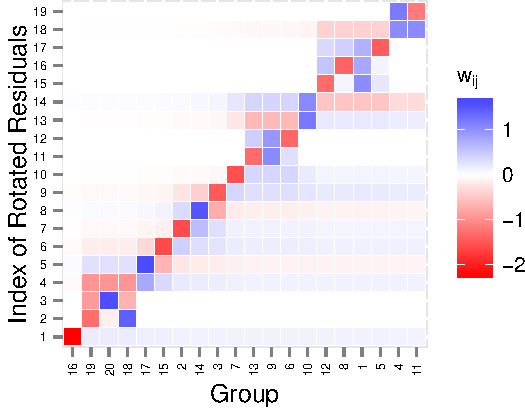
\includegraphics[width=0.4\textwidth]{cropped_cartoon_heatmap_raw.pdf}
	}
	\qquad
	\subfloat[$\bm{Q}\trans\bm{W}^{*\prime}$]{
		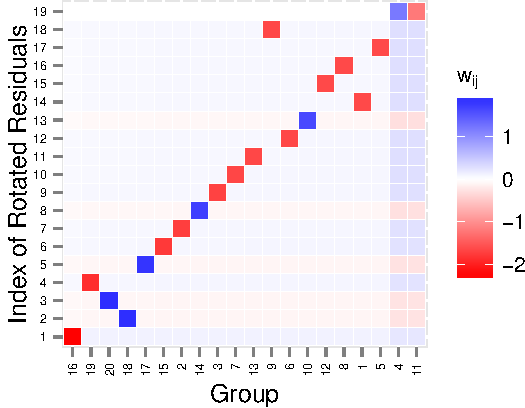
\includegraphics[width=0.4\textwidth]{cropped_cartoon_heatmap_varimax.pdf}
	}
	\caption{\label{fig:cartoon} Heatmap of $\bm{W}^{*\prime}$ and $\bm{Q}\trans\bm{W}^{*\prime}$ calculated where $\bm{Q}$ for a simulated random intercept model with 20 groups. Applying the varimax rotation, $\bm{Q}$, reduces the number of groups loading on a given rotated residual.}
\end{figure}

\paragraph{Extension to multiple random effects.}
Up to this point our discussion has ignored that a model may (and often will) contain numerous random effects. In this case, the assumptions made on each random effect should be checked; thus, we propose assessing the each random effect separately. To this end we must define linear combinations $\bm{L}_k$ such that $\bm{L}_k\trans \widehat{\bm{b}}$ produces the $k$th random effect. For example, in a model with a random intercept and random slope, if $\bm{Z}$ is organized as a block diagonal matrix---that is $\bm{Z} = \bigoplus_{i=1}^{m} \bm{Z}_{i}$ where $\bigoplus$ denotes the direct sum \citep[page 47]{Gentle:2007}---then $\bm{L}_0 = \bm{I}_{m} \bigotimes ( 1,\ 0)$ produces the random intercepts and $\bm{L}_1 = \bm{I}_{m} \bigotimes ( 0,\ 1)$ produces the random slopes. The methodology presented in this section can be generalized to models with numerous random effects by substituting $\bm{L}_k\trans \widehat{\bm{b}}$ for $\widehat{\bm{b}}$.


%----------------------------------------------------------------------------------
\section{Simulation study}\label{sec:simulation}
%----------------------------------------------------------------------------------

We conducted a simulation study to assess the specificity and sensitivity of tests of normality based on the two rotated residuals proposed in the previous section. 

\subsection{Design}\label{sec:sim-design}
%----------------------------------------------------------------------------------

The simulation study examined the proportion of Anderson-Darling (AD), Cram{\'e}r von Mises (CVM), and Kolmogorov-Smirnov (KS) tests for normality that rejected the null hypothesis of normality. This allows us to examine situations in which we correctly and incorrectly reject the null hypothesis of normality (i.e., power and type I error, respectively).  These test statistics measure the discrepancy between the empirical distribution of the rotated random effects and assumed distribution of the random effects, which sheds light on the behavior of Q-Q plots constructed from the rotated residuals. 

The design matrices from model \eqref{eq:radon} were used as templates for realistic data generation; however, only the 60 counties with full rank $\bm{Z}$ matrices were included for simplicity of the simulation design.
The following distributions were used to generate simulated residuals $\varepsilon_{ij}^*$, $b_{0i}^*$, and $b_{1i}^*$ from which the data were generated:
%
\begin{itemize}
\item $\varepsilon_{ij}^* \overset{iid}{\sim} \mathcal{N}(0, \ \sigma^2_{\varepsilon})$, or $\varepsilon_{ij}^* \overset{iid}{\sim} (\sigma_{\varepsilon} / \sqrt{3})\, t_3$ , or $\varepsilon_{ij}^* \overset{iid}{\sim} \sigma_{\varepsilon} \, \{ \text{Exp}(1) - 1 \}$

\item $b_{0i}^* \overset{iid}{\sim} \mathcal{N}(0, \ \sigma^2_{b_{0}})$, or $b_{0i}^* \overset{iid}{\sim} (\sigma_{b_{0}} / \sqrt{3})\, t_3$ , or $b_{0i}^* \overset{iid}{\sim} \sigma_{b_{0}} \, \{ \text{Exp}(1) - 1 \}$

\item $b_{1i}^* \overset{iid}{\sim} \mathcal{N}(0, \ \sigma^2_{b_{1}})$, or $b_{1i}^* \overset{iid}{\sim} (\sigma_{b_{1}} / \sqrt{3})\, t_3$ , or $b_{1i}^* \overset{iid}{\sim} \sigma_{b_{1}} \, \{ \text{Exp}(1) - 1 \}$
\end{itemize}
%
For simplicity we required the distributions of the random slope and intercept to the be same and assumed independence between the random effects. Additionally, the the fixed effects coefficients were set to the maximum likelihood estimates.

To investigate the effect that pooling has on the rotated random effects we considered  three variance structures:
%
\begin{itemize}
\item $\sigma^2_\varepsilon = 4$ and  $\sigma^2_{b_0} = \sigma^2_{b_1} = 1$
\item $\sigma^2_\varepsilon = 1$ and  $\sigma^2_{b_0} = \sigma^2_{b_1} = 1$
\item $\sigma^2_\varepsilon = 1$ and  $\sigma^2_{b_0} = \sigma^2_{b_1} = 4$

\end{itemize}
%

Under each simulation setting 1000 data sets were generated for each model and the rotated residuals were obtained using $s = \rank(\bm{B})$ (which are 58 and 59 for the random intercept and slope, respectively) as well as $s =$ 55, 50, 45, 40, 35, and 30.


\subsection{Results}\label{sec:sim-results}
%----------------------------------------------------------------------------------



\todo[inline]{Now summarize the results. Below is my informal summary (This is old now... ignore).}

\begin{itemize}
\item Overall, the rotated residuals reduce the type I error rates to rates much closer to the nominal level. When $\sigma^2_\varepsilon > \sigma^2_b$ there is minor inflation of the type I errors when the error terms are non-normal, but less severe than without the rotation. When $\sigma^2_\varepsilon \leq \sigma^2_b$ the type I errors are essentially at the nominal levels.

\item As expected, the power to detect non-normal random effects distributions is quite low for the rotated residuals. The varimax rotation does help amplify the power of detection, though an increase in the type I error rate also results.

\item The power to detect non-normal random effects distributions increases as $\sigma^2_b$ increases relative to $\sigma^2_\varepsilon$.


\end{itemize}

%----------------------------------------------------------------------------------
\section{Radon data: Revisited}\label{sec:radon2}
%----------------------------------------------------------------------------------

Now, we return to the motivating example and use rotated residuals to assess the distribution of the random effects.

\begin{itemize}
\item Show Q-Q plots for the rotated random effects
\item Discuss choice of $s$ in this example
\item Recap root of the problems with the raw random effects (errors not normally distributed; large degree of pooling/shrinkage)
\end{itemize}

%----------------------------------------------------------------------------------
\section{Discussion}\label{sec:discussion}
%----------------------------------------------------------------------------------

\todo[inline]{
Summarize everything and talk about future directions (if there are any). I have started a list below}
\begin{itemize}
\item Mention the robust model fitting procedures
\item Consideration of other orthogonal rotations (other than varimax)
\item Fact that we take for granted the estimation of the covariance matrices; thus some discussion of the future benefit of robust techniques would fit. A potential reference as a starting point is:\\ Li, E., \& Pourahmadi, M. (2013). An alternative REML estimation of covariance matrices in linear mixed models. Statistics \& Probability Letters, 83(4), 1071--1077. doi:10.1016/j.spl.2012.12.028
\item Discuss the relative speed of this procedure to a bootstrap procedure
\item Discuss why we are not using the ``upward'' residuals analysis approach discussed in the lit review chapter.
\end{itemize}

%----------------------------------------------------------------------------------
\section*{Appendix: Additional technical details}
%----------------------------------------------------------------------------------

We present the proof of the claim that the rotated residuals, $\bm{W}^{*\prime} \widehat{\bm{b}}$, are standardized, uncorrelated, and homoscedastic. Following the developments presented in Section~\ref{sec:rotate} we present this discussion for the random effects assuming that there is only a random intercept. Generalization to the situation with multiple random effects follows as previously discussed.

\begin{proof}
 Let $\bm{A} = \var(\widehat{\bm{b}} | \bm{b})$, $\bm{B} = \var(\widehat{\bm{b}})$, $r = \text{rank}(\bm{B})$, and $\ell = $ the number of elements in $\widehat{\bm{b}}$. Note that by definition $\bm{A}$ and $\bm{B}$ are symmetric and nonnegative definite. Following from above, $\bm{T}_r$ and $\bm{\Lambda}_r$ follow from the spectral (or eigenvalue) decomposition of $\bm{B} = \bm{T_r \Lambda_r T_r}\trans$, and $\bm{U}$ follows from the spectral decomposition of $\bm{A^*} = \bm{\Lambda_r}^{-1/2} \bm{T_r}\trans \bm{A T_r \Lambda_r}^{-1/2} = \bm{U} \bm{\Gamma} \bm{U}\trans$. Then, 
\begin{align*}
\var(\bm{W}^{*\prime} \widehat{\bm{b}}) &= \var(\bm{U}\trans \bm{\Lambda_r}^{-1/2} \bm{T_r}\trans \widehat{\bm{b}})\\
&= (\bm{U}\trans \bm{\Lambda_r}^{-1/2} \bm{T_r}\trans) \var(\widehat{\bm{b}}) (\bm{T_r \Lambda_r}^{-1/2} \bm{U})\\
&= (\bm{U}\trans \bm{\Lambda_r}^{-1/2} \bm{T_r}\trans) \bm{B} (\bm{T_r \Lambda_r}^{-1/2} \bm{U})\\
&= \bm{I}
\end{align*}
proving that the rotated errors are standardized, uncorrelated, and homoscedastic.
\end{proof}
 
%Recall that the trace of a matrix is equal to the sum of its eigenvalues; therefore, minimizing $\tr\left( \bm{B}\ginv\bm{A} \right)$ is equivalent to minimizing the sum of the eigenvalues of $\bm{B}\ginv\bm{A}$. The eigenvalues of $\bm{B}\ginv\bm{A}$ can be found through simultaneous diagonalization
% 
% 
%Write the spectral decomposition of $\bm{B}$ as
%$\bm{B} = \bm{T_r \Lambda_r T_r}\trans$, where $\bm{ \Lambda_r}$ is a diagonal matrix of the nonzero eigenvalues and $\bm{T_r}$ is the matrix of associated eigenvectors.
%Define $\bm{F} = \bm{T_r \Lambda_r}^{1/2}$, which is a full-rank decomposition of $\bm{B}$. The Moore-Penrose inverse of $\bm{F}$ is given by
%\[
%\bm{F}\ginv = (\bm{F}\trans\bm{F})\inv \bm{F}\trans = \bm{\Lambda_r}^{-1/2} \bm{T_r}\trans
%\]
%Now, notice that
%\[
%\bm{F}\ginv \bm{B} (\bm{F}\ginv)\trans = \bm{\Lambda_r}^{-1/2} \bm{T_r}\trans ( \bm{T_r \Lambda_r T_r}\trans ) \bm{T_r \Lambda_r}^{-1/2} =  \bm{I}
%\]
%and define
%\[
%	\bm{A}^* = \bm{F}\ginv \bm{A} (\bm{F}\ginv)\trans
%\]
%Next, we rewrite $\bm{W} = (\bm{F}\ginv)\trans \bm{U}$, where $\bm{U}$ is a nonsingular symmetric matrix. Then \eqref{eq:app1} becomes
%%
%\begin{equation}\label{eq:app2}
%\tr \left[ \left( \bm{U}\trans \bm{F}\ginv \bm{B} (\bm{F}\ginv)\trans \bm{U} \right)\inv 
%\left(\bm{U}\trans \bm{F}\ginv \bm{A} (\bm{F}\ginv)\trans \bm{U} \right) \right]
%=
%\tr \left[ \left( \bm{U}\trans \bm{I} \bm{U} \right)\inv \left( \bm{U}\trans \bm{A}^* \bm{U} \right) \right]
%\end{equation}
%%
%whose derivative with respect to $\bm{U}$ is given by
%%
%\begin{equation}\label{eq:app3}
%-2 \bm{IU} \left( \bm{U}\trans \bm{I} \bm{U} \right)\inv \left( \bm{U}\trans \bm{A}^* \bm{U} \right) \left( \bm{U}\trans \bm{I} \bm{U} \right)\inv + 2 \bm{A}^* \bm{U} \left( \bm{U}\trans \bm{I} \bm{U} \right)\inv
%\end{equation}
%%
%\citep[A.16]{Fukunaga:1990}. Setting \eqref{eq:app3} to zero we find that the solution must satisfy
%%
%\begin{equation}
%\bm{A}^* \bm{U} = \bm{U} \left( \bm{U}\trans \bm{A}^* \bm{U} \right)
%\end{equation}
%%
%
%
%which is of the form of an eigenvalue problem, which is minimized at the eigenvector corresponding to the smallest eigenvalue of  $\bm{A}^*$. Additionally, the value of \eqref{eq:app2} lies between the minimum and maximum eigenvalue of $\bm{A}^*$.
%
%The requirement that $\bm{W}$ be of full rank results in $\bm{W} = \bm{T_r \Lambda_r}^{-1/2} \bm{U}$, where $\bm{U}$ are the eigenvectors of $\bm{A}^*$.
%\end{proof}
%
%More general proofs can be found in \cite{McDonald:1979ca} and \cite{deLeeuw:1982to}.
%
%Next we show that the resulting residuals are standardized, uncorrelated, and homoscedastic.
%
%\begin{proof} Carrying through the notation from above we see that
%\begin{align*}
%\var(\bm{W}^{*\prime} \widehat{\bm{e}}) &= \var(\bm{U}\trans \bm{\Lambda_r}^{-1/2} \bm{T_r}\trans \widehat{\bm{e}})\\
%&= (\bm{U}\trans \bm{\Lambda_r}^{-1/2} \bm{T_r}\trans) \var(\widehat{\bm{e}}) (\bm{T_r \Lambda_r}^{-1/2} \bm{U})\\
%&= (\bm{U}\trans \bm{\Lambda_r}^{-1/2} \bm{T_r}\trans) \bm{B} (\bm{T_r \Lambda_r}^{-1/2} \bm{U})\\
%&= \bm{I}
%\end{align*}
%
%\end{proof}


%----------------------------------------------------------------------------------
%----------------------------------------------------------------------------------
\bibliographystyle{apa}
\bibliography{lcresid_bib}
%----------------------------------------------------------------------------------
%----------------------------------------------------------------------------------

\clearpage

%----------------------------------------------------------------------------------
\appendix
\section{Supplement to ``Are you Normal? The Problem of Confounded Residual Structures in Hierarchical Linear Models''}
%----------------------------------------------------------------------------------

\subsection{Full simulation results}

\begin{table}[ht]
\caption{Tests for normality of the random intercept using two rotations and $s = \rank(\bm{B})$.}
\begin{scriptsize}
\begin{center}
\begin{tabular}{ll p{.1cm} c p{.1cm} rrr p{.1cm} rrr}
  \hline
  \multicolumn{2}{c}{Distributions}& & Nominal & &  \multicolumn{3}{c}{Rotation} & & \multicolumn{3}{c}{Varimax rotation} \\ \cline{1-2} \cline{6-8} \cline{10-12}   
  Random effects & Errors & & $\alpha$ & & AD & CVM & KS & & AD & CVM & KS \\ 
   \hline
& && && \multicolumn{7}{c}{$\sigma_{\varepsilon}^2 = 4$, \ \ $\sigma_{b_0}^2 = \sigma_{b_1}^2 = 1$} \\ \cline{6-12}
Normal       & Normal       && 0.05 &&   0.04 & 0.04 & 0.04 && 0.05 & 0.05 & 0.06 \\ 
             &              && 0.10 &&   0.10 & 0.10 & 0.10 && 0.11 & 0.11 & 0.11 \\ 
             & Heavy tailed && 0.05 &&   0.07 & 0.07 & 0.07 && 0.09 & 0.08 & 0.07 \\ 
             &              && 0.10 &&   0.13 & 0.13 & 0.13 && 0.16 & 0.15 & 0.14 \\ 
             & Skewed       && 0.05 &&   0.05 & 0.05 & 0.05 && 0.05 & 0.05 & 0.05 \\ 
             &              && 0.10 &&   0.10 & 0.09 & 0.09 && 0.10 & 0.10 & 0.11 \\ 
Heavy tailed & Normal       && 0.05 &&   0.14 & 0.13 & 0.10 && 0.22 & 0.20 & 0.17 \\ 
             &              && 0.10 &&   0.20 & 0.19 & 0.18 && 0.31 & 0.28 & 0.24 \\ 
             & Heavy tailed && 0.05 &&   0.19 & 0.17 & 0.15 && 0.34 & 0.32 & 0.26 \\ 
             &              && 0.10 &&   0.26 & 0.24 & 0.21 && 0.44 & 0.41 & 0.35 \\ 
             & Skewed       && 0.05 &&   0.15 & 0.14 & 0.13 && 0.28 & 0.23 & 0.20 \\ 
             &              && 0.10 &&   0.21 & 0.18 & 0.18 && 0.37 & 0.32 & 0.28 \\ 
Skewed       & Normal       && 0.05 &&   0.10 & 0.09 & 0.08 && 0.20 & 0.17 & 0.12 \\ 
             &              && 0.10 &&   0.17 & 0.15 & 0.15 && 0.29 & 0.25 & 0.19 \\ 
             & Heavy tailed && 0.05 &&   0.13 & 0.11 & 0.11 && 0.30 & 0.24 & 0.19 \\ 
             &              && 0.10 &&   0.22 & 0.19 & 0.17 && 0.39 & 0.34 & 0.28 \\ 
             & Skewed       && 0.05 &&   0.13 & 0.12 & 0.09 && 0.22 & 0.19 & 0.15 \\ 
             &              && 0.10 &&   0.19 & 0.17 & 0.16 && 0.33 & 0.28 & 0.25 \\ 

&&&&&&&&&&&\\
& && && \multicolumn{7}{c}{$\sigma_{\varepsilon}^2 = 1$, \ \ $\sigma_{b_0}^2 = \sigma_{b_1}^2 = 1$} \\ \cline{6-12}
Normal       & Normal       && 0.05 &&   0.05 & 0.05 & 0.04 && 0.05 & 0.06 & 0.05 \\ 
             &              && 0.10 &&   0.09 & 0.09 & 0.09 && 0.11 & 0.11 & 0.12 \\ 
             & Heavy tailed && 0.05 &&   0.06 & 0.07 & 0.06 && 0.06 & 0.06 & 0.05 \\ 
             &              && 0.10 &&   0.11 & 0.10 & 0.11 && 0.11 & 0.11 & 0.11 \\ 
             & Skewed       && 0.05 &&   0.05 & 0.04 & 0.04 && 0.05 & 0.05 & 0.04 \\ 
             &              && 0.10 &&   0.09 & 0.09 & 0.09 && 0.10 & 0.10 & 0.09 \\ 
Heavy tailed & Normal       && 0.05 &&   0.21 & 0.20 & 0.16 && 0.40 & 0.35 & 0.28 \\ 
             &              && 0.10 &&   0.29 & 0.27 & 0.23 && 0.49 & 0.45 & 0.39 \\ 
             & Heavy tailed && 0.05 &&   0.25 & 0.22 & 0.17 && 0.47 & 0.42 & 0.34 \\ 
             &              && 0.10 &&   0.32 & 0.30 & 0.25 && 0.54 & 0.50 & 0.44 \\ 
             & Skewed       && 0.05 &&   0.25 & 0.22 & 0.17 && 0.42 & 0.38 & 0.30 \\ 
             &              && 0.10 &&   0.33 & 0.30 & 0.27 && 0.50 & 0.46 & 0.40 \\ 
Skewed       & Normal       && 0.05 &&   0.17 & 0.16 & 0.13 && 0.36 & 0.28 & 0.21 \\ 
             &              && 0.10 &&   0.26 & 0.24 & 0.20 && 0.47 & 0.38 & 0.31 \\ 
             & Heavy tailed && 0.05 &&   0.20 & 0.18 & 0.14 && 0.42 & 0.34 & 0.25 \\ 
             &              && 0.10 &&   0.28 & 0.26 & 0.23 && 0.51 & 0.44 & 0.35 \\ 
             & Skewed       && 0.05 &&   0.18 & 0.17 & 0.12 && 0.40 & 0.30 & 0.21 \\ 
             &              && 0.10 &&   0.26 & 0.23 & 0.22 && 0.51 & 0.39 & 0.33 \\ 

&&&&&&&&&&&\\
& && && \multicolumn{7}{c}{$\sigma_{\varepsilon}^2 = 1$, \ \ $\sigma_{b_0}^2 = \sigma_{b_1}^2 = 4$} \\ \cline{6-12}

\hline
\end{tabular}
\end{center}
\end{scriptsize}
\end{table}


\begin{table}[ht]
\caption{Tests for normality of the random intercept using two rotations and $s = 55$.}
\begin{scriptsize}
\begin{center}
\begin{tabular}{ll p{.1cm} c p{.1cm} rrr p{.1cm} rrr}
  \hline
  \multicolumn{2}{c}{Distributions}& & Nominal & &  \multicolumn{3}{c}{Rotation} & & \multicolumn{3}{c}{Varimax rotation} \\ \cline{1-2} \cline{6-8} \cline{10-12}   
  Random effects & Errors & & $\alpha$ & & AD & CVM & KS & & AD & CVM & KS \\ 
   \hline
& && && \multicolumn{7}{c}{$\sigma_{\varepsilon}^2 = 4$, \ \ $\sigma_{b_0}^2 = \sigma_{b_1}^2 = 1$} \\ \cline{6-12}
Normal       & Normal       && 0.05 &&   0.04 & 0.04 & 0.04 && 0.05 & 0.06 & 0.05 \\ 
             &              && 0.10 &&   0.09 & 0.09 & 0.10 && 0.10 & 0.10 & 0.11 \\ 
             & Heavy tailed && 0.05 &&   0.08 & 0.08 & 0.06 && 0.09 & 0.08 & 0.08 \\ 
             &              && 0.10 &&   0.13 & 0.14 & 0.12 && 0.17 & 0.15 & 0.13 \\ 
             & Skewed       && 0.05 &&   0.05 & 0.05 & 0.05 && 0.05 & 0.05 & 0.05 \\ 
             &              && 0.10 &&   0.09 & 0.09 & 0.10 && 0.09 & 0.09 & 0.11 \\ 
Heavy tailed & Normal       && 0.05 &&   0.14 & 0.12 & 0.11 && 0.22 & 0.20 & 0.17 \\ 
             &              && 0.10 &&   0.20 & 0.20 & 0.18 && 0.30 & 0.27 & 0.23 \\ 
             & Heavy tailed && 0.05 &&   0.19 & 0.17 & 0.14 && 0.33 & 0.32 & 0.25 \\ 
             &              && 0.10 &&   0.25 & 0.23 & 0.21 && 0.45 & 0.40 & 0.34 \\ 
             & Skewed       && 0.05 &&   0.15 & 0.14 & 0.11 && 0.27 & 0.21 & 0.17 \\ 
             &              && 0.10 &&   0.21 & 0.19 & 0.19 && 0.36 & 0.32 & 0.27 \\ 
Skewed       & Normal       && 0.05 &&   0.09 & 0.08 & 0.08 && 0.21 & 0.17 & 0.12 \\ 
             &              && 0.10 &&   0.16 & 0.14 & 0.14 && 0.29 & 0.24 & 0.20 \\ 
             & Heavy tailed && 0.05 &&   0.12 & 0.11 & 0.10 && 0.28 & 0.24 & 0.18 \\ 
             &              && 0.10 &&   0.20 & 0.18 & 0.17 && 0.38 & 0.33 & 0.27 \\ 
             & Skewed       && 0.05 &&   0.13 & 0.12 & 0.10 && 0.23 & 0.19 & 0.15 \\ 
             &              && 0.10 &&   0.18 & 0.17 & 0.15 && 0.32 & 0.28 & 0.24 \\ 

&&&&&&&&&&&\\
& && && \multicolumn{7}{c}{$\sigma_{\varepsilon}^2 = 1$, \ \ $\sigma_{b_0}^2 = \sigma_{b_1}^2 = 1$} \\ \cline{6-12}
Normal       & Normal       && 0.05 &&   0.04 & 0.05 & 0.04 && 0.04 & 0.05 & 0.05 \\ 
             &              && 0.10 &&   0.10 & 0.09 & 0.09 && 0.10 & 0.10 & 0.10 \\ 
             & Heavy tailed && 0.05 &&   0.06 & 0.06 & 0.05 && 0.06 & 0.05 & 0.04 \\ 
             &              && 0.10 &&   0.10 & 0.10 & 0.11 && 0.11 & 0.10 & 0.10 \\ 
             & Skewed       && 0.05 &&   0.04 & 0.03 & 0.03 && 0.05 & 0.05 & 0.04 \\ 
             &              && 0.10 &&   0.09 & 0.08 & 0.07 && 0.10 & 0.09 & 0.09 \\ 
Heavy tailed & Normal       && 0.05 &&   0.19 & 0.18 & 0.15 && 0.39 & 0.36 & 0.30 \\ 
             &              && 0.10 &&   0.28 & 0.25 & 0.23 && 0.49 & 0.45 & 0.39 \\ 
             & Heavy tailed && 0.05 &&   0.24 & 0.23 & 0.18 && 0.44 & 0.40 & 0.33 \\ 
             &              && 0.10 &&   0.31 & 0.30 & 0.26 && 0.53 & 0.49 & 0.42 \\ 
             & Skewed       && 0.05 &&   0.24 & 0.21 & 0.17 && 0.41 & 0.36 & 0.28 \\ 
             &              && 0.10 &&   0.32 & 0.30 & 0.25 && 0.49 & 0.45 & 0.38 \\ 
Skewed       & Normal       && 0.05 &&   0.17 & 0.17 & 0.14 && 0.36 & 0.28 & 0.22 \\ 
             &              && 0.10 &&   0.27 & 0.24 & 0.20 && 0.47 & 0.38 & 0.32 \\ 
             & Heavy tailed && 0.05 &&   0.20 & 0.17 & 0.14 && 0.41 & 0.34 & 0.25 \\ 
             &              && 0.10 &&   0.29 & 0.27 & 0.22 && 0.51 & 0.42 & 0.34 \\ 
             & Skewed       && 0.05 &&   0.18 & 0.16 & 0.12 && 0.40 & 0.30 & 0.21 \\ 
             &              && 0.10 &&   0.24 & 0.22 & 0.21 && 0.52 & 0.40 & 0.33 \\ 


&&&&&&&&&&&\\
& && && \multicolumn{7}{c}{$\sigma_{\varepsilon}^2 = 1$, \ \ $\sigma_{b_0}^2 = \sigma_{b_1}^2 = 4$} \\ \cline{6-12}
Normal       & Normal       && 0.05 &&   0.05 & 0.05 & 0.05 && 0.05 & 0.05 & 0.03 \\ 
             &              && 0.10 &&   0.10 & 0.11 & 0.11 && 0.09 & 0.10 & 0.10 \\ 
             & Heavy tailed && 0.05 &&   0.07 & 0.07 & 0.06 && 0.05 & 0.05 & 0.06 \\ 
             &              && 0.10 &&   0.13 & 0.12 & 0.11 && 0.10 & 0.10 & 0.10 \\ 
             & Skewed       && 0.05 &&   0.05 & 0.04 & 0.04 && 0.05 & 0.05 & 0.05 \\ 
             &              && 0.10 &&   0.10 & 0.10 & 0.10 && 0.09 & 0.09 & 0.10 \\ 
Heavy tailed & Normal       && 0.05 &&   0.27 & 0.24 & 0.20 && 0.42 & 0.37 & 0.29 \\ 
             &              && 0.10 &&   0.33 & 0.31 & 0.28 && 0.51 & 0.47 & 0.39 \\ 
             & Heavy tailed && 0.05 &&   0.28 & 0.25 & 0.22 && 0.43 & 0.39 & 0.31 \\ 
             &              && 0.10 &&   0.37 & 0.35 & 0.28 && 0.52 & 0.48 & 0.42 \\ 
             & Skewed       && 0.05 &&   0.27 & 0.24 & 0.20 && 0.42 & 0.37 & 0.28 \\ 
             &              && 0.10 &&   0.35 & 0.32 & 0.28 && 0.51 & 0.47 & 0.39 \\ 
Skewed       & Normal       && 0.05 &&   0.23 & 0.21 & 0.15 && 0.37 & 0.29 & 0.21 \\ 
             &              && 0.10 &&   0.31 & 0.29 & 0.24 && 0.46 & 0.38 & 0.31 \\ 
             & Heavy tailed && 0.05 &&   0.23 & 0.21 & 0.17 && 0.35 & 0.27 & 0.21 \\ 
             &              && 0.10 &&   0.33 & 0.32 & 0.26 && 0.44 & 0.37 & 0.30 \\ 
             & Skewed       && 0.05 &&   0.23 & 0.21 & 0.16 && 0.38 & 0.28 & 0.21 \\ 
             &              && 0.10 &&   0.32 & 0.30 & 0.26 && 0.47 & 0.38 & 0.31 \\ 

\hline
\end{tabular}
\end{center}
\end{scriptsize}
\end{table}


\begin{table}[ht]
\caption{Tests for normality of the random intercept using two rotations and $s = 50$.}
\begin{scriptsize}
\begin{center}
\begin{tabular}{ll p{.1cm} c p{.1cm} rrr p{.1cm} rrr}
  \hline
  \multicolumn{2}{c}{Distributions}& & Nominal & &  \multicolumn{3}{c}{Rotation} & & \multicolumn{3}{c}{Varimax rotation} \\ \cline{1-2} \cline{6-8} \cline{10-12}   
  Random effects & Errors & & $\alpha$ & & AD & CVM & KS & & AD & CVM & KS \\ 
   \hline
& && && \multicolumn{7}{c}{$\sigma_{\varepsilon}^2 = 4$, \ \ $\sigma_{b_0}^2 = \sigma_{b_1}^2 = 1$} \\ \cline{6-12}
Normal       & Normal       && 0.05 &&   0.05 & 0.05 & 0.05 && 0.05 & 0.06 & 0.06 \\ 
             &              && 0.10 &&   0.11 & 0.10 & 0.10 && 0.11 & 0.11 & 0.11 \\ 
             & Heavy tailed && 0.05 &&   0.07 & 0.07 & 0.07 && 0.08 & 0.08 & 0.07 \\ 
             &              && 0.10 &&   0.12 & 0.13 & 0.12 && 0.14 & 0.13 & 0.13 \\ 
             & Skewed       && 0.05 &&   0.06 & 0.06 & 0.05 && 0.04 & 0.04 & 0.04 \\ 
             &              && 0.10 &&   0.11 & 0.10 & 0.10 && 0.09 & 0.09 & 0.10 \\ 
Heavy tailed & Normal       && 0.05 &&   0.13 & 0.12 & 0.10 && 0.23 & 0.20 & 0.15 \\ 
             &              && 0.10 &&   0.20 & 0.18 & 0.17 && 0.31 & 0.27 & 0.24 \\ 
             & Heavy tailed && 0.05 &&   0.17 & 0.16 & 0.13 && 0.32 & 0.28 & 0.22 \\ 
             &              && 0.10 &&   0.24 & 0.23 & 0.20 && 0.41 & 0.38 & 0.32 \\ 
             & Skewed       && 0.05 &&   0.14 & 0.13 & 0.12 && 0.26 & 0.22 & 0.18 \\ 
             &              && 0.10 &&   0.21 & 0.19 & 0.18 && 0.35 & 0.31 & 0.28 \\ 
Skewed       & Normal       && 0.05 &&   0.10 & 0.08 & 0.08 && 0.21 & 0.17 & 0.12 \\ 
             &              && 0.10 &&   0.16 & 0.15 & 0.14 && 0.31 & 0.27 & 0.19 \\ 
             & Heavy tailed && 0.05 &&   0.12 & 0.11 & 0.09 && 0.27 & 0.22 & 0.17 \\ 
             &              && 0.10 &&   0.20 & 0.17 & 0.16 && 0.37 & 0.31 & 0.25 \\ 
             & Skewed       && 0.05 &&   0.12 & 0.11 & 0.09 && 0.22 & 0.18 & 0.14 \\ 
             &              && 0.10 &&   0.19 & 0.17 & 0.15 && 0.31 & 0.26 & 0.23 \\ 

&&&&&&&&&&&\\
& && && \multicolumn{7}{c}{$\sigma_{\varepsilon}^2 = 1$, \ \ $\sigma_{b_0}^2 = \sigma_{b_1}^2 = 1$} \\ \cline{6-12}
Normal       & Normal       && 0.05 &&   0.04 & 0.05 & 0.04 && 0.04 & 0.05 & 0.05 \\ 
             &              && 0.10 &&   0.09 & 0.09 & 0.08 && 0.10 & 0.10 & 0.10 \\ 
             & Heavy tailed && 0.05 &&   0.06 & 0.06 & 0.05 && 0.06 & 0.06 & 0.06 \\ 
             &              && 0.10 &&   0.10 & 0.11 & 0.11 && 0.12 & 0.12 & 0.10 \\ 
             & Skewed       && 0.05 &&   0.04 & 0.04 & 0.03 && 0.05 & 0.04 & 0.04 \\ 
             &              && 0.10 &&   0.09 & 0.08 & 0.08 && 0.08 & 0.08 & 0.09 \\ 
Heavy tailed & Normal       && 0.05 &&   0.18 & 0.17 & 0.14 && 0.39 & 0.36 & 0.30 \\ 
             &              && 0.10 &&   0.27 & 0.24 & 0.23 && 0.47 & 0.43 & 0.40 \\ 
             & Heavy tailed && 0.05 &&   0.23 & 0.21 & 0.17 && 0.43 & 0.38 & 0.31 \\ 
             &              && 0.10 &&   0.31 & 0.28 & 0.25 && 0.52 & 0.48 & 0.41 \\ 
             & Skewed       && 0.05 &&   0.24 & 0.21 & 0.16 && 0.41 & 0.37 & 0.29 \\ 
             &              && 0.10 &&   0.31 & 0.29 & 0.24 && 0.50 & 0.45 & 0.38 \\ 
Skewed       & Normal       && 0.05 &&   0.18 & 0.16 & 0.12 && 0.34 & 0.28 & 0.20 \\ 
             &              && 0.10 &&   0.25 & 0.23 & 0.21 && 0.46 & 0.38 & 0.31 \\ 
             & Heavy tailed && 0.05 &&   0.19 & 0.18 & 0.15 && 0.40 & 0.31 & 0.24 \\ 
             &              && 0.10 &&   0.28 & 0.26 & 0.23 && 0.49 & 0.42 & 0.35 \\ 
             & Skewed       && 0.05 &&   0.17 & 0.15 & 0.11 && 0.37 & 0.27 & 0.22 \\ 
             &              && 0.10 &&   0.24 & 0.22 & 0.19 && 0.47 & 0.38 & 0.33 \\ 


&&&&&&&&&&&\\
& && && \multicolumn{7}{c}{$\sigma_{\varepsilon}^2 = 1$, \ \ $\sigma_{b_0}^2 = \sigma_{b_1}^2 = 4$} \\ \cline{6-12}

\hline
\end{tabular}
\end{center}
\end{scriptsize}
\end{table}

\begin{table}[ht]
\caption{Tests for normality of the random intercept using two rotations and $s = 45$.}
\begin{scriptsize}
\begin{center}
\begin{tabular}{ll p{.1cm} c p{.1cm} rrr p{.1cm} rrr}
  \hline
  \multicolumn{2}{c}{Distributions}& & Nominal & &  \multicolumn{3}{c}{Rotation} & & \multicolumn{3}{c}{Varimax rotation} \\ \cline{1-2} \cline{6-8} \cline{10-12}   
  Random effects & Errors & & $\alpha$ & & AD & CVM & KS & & AD & CVM & KS \\ 
   \hline
& && && \multicolumn{7}{c}{$\sigma_{\varepsilon}^2 = 4$, \ \ $\sigma_{b_0}^2 = \sigma_{b_1}^2 = 1$} \\ \cline{6-12}
Normal       & Normal       && 0.05 &&   0.04 & 0.04 & 0.04 && 0.05 & 0.06 & 0.05 \\ 
             &              && 0.10 &&   0.10 & 0.10 & 0.10 && 0.11 & 0.10 & 0.10 \\ 
             & Heavy tailed && 0.05 &&   0.06 & 0.06 & 0.06 && 0.07 & 0.07 & 0.06 \\ 
             &              && 0.10 &&   0.12 & 0.12 & 0.12 && 0.13 & 0.12 & 0.10 \\ 
             & Skewed       && 0.05 &&   0.06 & 0.06 & 0.05 && 0.06 & 0.05 & 0.04 \\ 
             &              && 0.10 &&   0.10 & 0.10 & 0.09 && 0.11 & 0.10 & 0.09 \\ 
Heavy tailed & Normal       && 0.05 &&   0.13 & 0.12 & 0.10 && 0.23 & 0.21 & 0.15 \\ 
             &              && 0.10 &&   0.20 & 0.18 & 0.18 && 0.30 & 0.27 & 0.24 \\ 
             & Heavy tailed && 0.05 &&   0.16 & 0.15 & 0.13 && 0.32 & 0.27 & 0.22 \\ 
             &              && 0.10 &&   0.23 & 0.22 & 0.19 && 0.40 & 0.37 & 0.32 \\ 
             & Skewed       && 0.05 &&   0.14 & 0.13 & 0.11 && 0.27 & 0.24 & 0.18 \\ 
             &              && 0.10 &&   0.21 & 0.19 & 0.17 && 0.34 & 0.31 & 0.28 \\ 
Skewed       & Normal       && 0.05 &&   0.10 & 0.10 & 0.08 && 0.22 & 0.20 & 0.14 \\ 
             &              && 0.10 &&   0.18 & 0.16 & 0.14 && 0.31 & 0.26 & 0.22 \\ 
             & Heavy tailed && 0.05 &&   0.11 & 0.10 & 0.10 && 0.25 & 0.20 & 0.16 \\ 
             &              && 0.10 &&   0.18 & 0.17 & 0.15 && 0.35 & 0.30 & 0.25 \\ 
             & Skewed       && 0.05 &&   0.12 & 0.11 & 0.10 && 0.23 & 0.20 & 0.14 \\ 
             &              && 0.10 &&   0.19 & 0.18 & 0.16 && 0.32 & 0.27 & 0.20 \\ 

&&&&&&&&&&&\\
& && && \multicolumn{7}{c}{$\sigma_{\varepsilon}^2 = 1$, \ \ $\sigma_{b_0}^2 = \sigma_{b_1}^2 = 1$} \\ \cline{6-12}
Normal       & Normal       && 0.05 &&   0.04 & 0.04 & 0.04 && 0.04 & 0.05 & 0.05 \\ 
             &              && 0.10 &&   0.09 & 0.09 & 0.09 && 0.10 & 0.10 & 0.11 \\ 
             & Heavy tailed && 0.05 &&   0.06 & 0.06 & 0.05 && 0.05 & 0.06 & 0.05 \\ 
             &              && 0.10 &&   0.10 & 0.10 & 0.10 && 0.12 & 0.11 & 0.10 \\ 
             & Skewed       && 0.05 &&   0.04 & 0.04 & 0.04 && 0.06 & 0.06 & 0.05 \\ 
             &              && 0.10 &&   0.09 & 0.08 & 0.08 && 0.10 & 0.10 & 0.11 \\ 
Heavy tailed & Normal       && 0.05 &&   0.18 & 0.17 & 0.14 && 0.37 & 0.33 & 0.28 \\ 
             &              && 0.10 &&   0.26 & 0.24 & 0.22 && 0.45 & 0.41 & 0.37 \\ 
             & Heavy tailed && 0.05 &&   0.21 & 0.20 & 0.14 && 0.40 & 0.36 & 0.27 \\ 
             &              && 0.10 &&   0.28 & 0.26 & 0.23 && 0.49 & 0.45 & 0.38 \\ 
             & Skewed       && 0.05 &&   0.22 & 0.19 & 0.16 && 0.39 & 0.34 & 0.27 \\ 
             &              && 0.10 &&   0.28 & 0.26 & 0.23 && 0.47 & 0.43 & 0.37 \\ 
Skewed       & Normal       && 0.05 &&   0.17 & 0.15 & 0.12 && 0.36 & 0.28 & 0.23 \\ 
             &              && 0.10 &&   0.25 & 0.24 & 0.19 && 0.45 & 0.38 & 0.31 \\ 
             & Heavy tailed && 0.05 &&   0.19 & 0.17 & 0.14 && 0.38 & 0.32 & 0.24 \\ 
             &              && 0.10 &&   0.27 & 0.24 & 0.22 && 0.48 & 0.41 & 0.34 \\ 
             & Skewed       && 0.05 &&   0.15 & 0.13 & 0.10 && 0.34 & 0.26 & 0.20 \\ 
             &              && 0.10 &&   0.22 & 0.20 & 0.16 && 0.47 & 0.38 & 0.30 \\ 


&&&&&&&&&&&\\
& && && \multicolumn{7}{c}{$\sigma_{\varepsilon}^2 = 1$, \ \ $\sigma_{b_0}^2 = \sigma_{b_1}^2 = 4$} \\ \cline{6-12}
Normal       & Normal       && 0.05 &&   0.05 & 0.05 & 0.05 && 0.05 & 0.06 & 0.06 \\ 
             &              && 0.10 &&   0.11 & 0.11 & 0.09 && 0.11 & 0.10 & 0.11 \\ 
             & Heavy tailed && 0.05 &&   0.06 & 0.06 & 0.06 && 0.05 & 0.05 & 0.04 \\ 
             &              && 0.10 &&   0.12 & 0.12 & 0.11 && 0.09 & 0.09 & 0.09 \\ 
             & Skewed       && 0.05 &&   0.05 & 0.05 & 0.05 && 0.06 & 0.06 & 0.05 \\ 
             &              && 0.10 &&   0.10 & 0.10 & 0.11 && 0.11 & 0.11 & 0.11 \\ 
Heavy tailed & Normal       && 0.05 &&   0.22 & 0.20 & 0.18 && 0.36 & 0.32 & 0.25 \\ 
             &              && 0.10 &&   0.30 & 0.28 & 0.24 && 0.48 & 0.43 & 0.35 \\ 
             & Heavy tailed && 0.05 &&   0.24 & 0.23 & 0.17 && 0.37 & 0.35 & 0.29 \\ 
             &              && 0.10 &&   0.32 & 0.31 & 0.26 && 0.46 & 0.43 & 0.37 \\ 
             & Skewed       && 0.05 &&   0.24 & 0.23 & 0.17 && 0.37 & 0.34 & 0.26 \\ 
             &              && 0.10 &&   0.33 & 0.30 & 0.26 && 0.46 & 0.44 & 0.35 \\ 
Skewed       & Normal       && 0.05 &&   0.21 & 0.20 & 0.14 && 0.34 & 0.27 & 0.21 \\ 
             &              && 0.10 &&   0.30 & 0.30 & 0.23 && 0.44 & 0.36 & 0.29 \\ 
             & Heavy tailed && 0.05 &&   0.22 & 0.22 & 0.16 && 0.33 & 0.25 & 0.20 \\ 
             &              && 0.10 &&   0.31 & 0.30 & 0.26 && 0.43 & 0.36 & 0.28 \\ 
             & Skewed       && 0.05 &&   0.21 & 0.21 & 0.17 && 0.33 & 0.24 & 0.19 \\ 
             &              && 0.10 &&   0.29 & 0.27 & 0.25 && 0.43 & 0.34 & 0.28 \\ 

\hline
\end{tabular}
\end{center}
\end{scriptsize}
\end{table}

\begin{table}[ht]
\caption{Tests for normality of the random intercept using two rotations and $s = 40$.}
\begin{scriptsize}
\begin{center}
\begin{tabular}{ll p{.1cm} c p{.1cm} rrr p{.1cm} rrr}
  \hline
  \multicolumn{2}{c}{Distributions}& & Nominal & &  \multicolumn{3}{c}{Rotation} & & \multicolumn{3}{c}{Varimax rotation} \\ \cline{1-2} \cline{6-8} \cline{10-12}   
  Random effects & Errors & & $\alpha$ & & AD & CVM & KS & & AD & CVM & KS \\ 
   \hline
& && && \multicolumn{7}{c}{$\sigma_{\varepsilon}^2 = 4$, \ \ $\sigma_{b_0}^2 = \sigma_{b_1}^2 = 1$} \\ \cline{6-12}
Normal       & Normal       && 0.05 &&   0.04 & 0.05 & 0.04 & 0.05 & 0.05 & 0.06 \\ 
             &              && 0.10 &&   0.11 & 0.10 & 0.09 & 0.12 & 0.12 & 0.11 \\ 
             & Heavy tailed && 0.05 &&   0.05 & 0.05 & 0.06 & 0.06 & 0.06 & 0.04 \\ 
             &              && 0.10 &&   0.11 & 0.11 & 0.12 & 0.12 & 0.12 & 0.10 \\ 
             & Skewed       && 0.05 &&   0.06 & 0.06 & 0.05 & 0.06 & 0.06 & 0.06 \\ 
             &              && 0.10 &&   0.11 & 0.11 & 0.10 & 0.12 & 0.11 & 0.11 \\ 
Heavy tailed & Normal       && 0.05 &&   0.13 & 0.12 & 0.10 & 0.23 & 0.20 & 0.17 \\ 
             &              && 0.10 &&   0.21 & 0.19 & 0.18 & 0.31 & 0.29 & 0.25 \\ 
             & Heavy tailed && 0.05 &&   0.16 & 0.15 & 0.11 & 0.30 & 0.27 & 0.22 \\ 
             &              && 0.10 &&   0.23 & 0.21 & 0.20 & 0.38 & 0.35 & 0.30 \\ 
             & Skewed       && 0.05 &&   0.13 & 0.12 & 0.10 & 0.24 & 0.22 & 0.17 \\ 
             &              && 0.10 &&   0.20 & 0.17 & 0.16 & 0.31 & 0.29 & 0.26 \\ 
Skewed       & Normal       && 0.05 &&   0.10 & 0.08 & 0.08 & 0.23 & 0.18 & 0.15 \\ 
             &              && 0.10 &&   0.18 & 0.17 & 0.14 & 0.32 & 0.27 & 0.23 \\ 
             & Heavy tailed && 0.05 &&   0.10 & 0.09 & 0.08 & 0.26 & 0.21 & 0.16 \\ 
             &              && 0.10 &&   0.18 & 0.16 & 0.14 & 0.35 & 0.29 & 0.25 \\ 
             & Skewed       && 0.05 &&   0.11 & 0.11 & 0.10 & 0.21 & 0.17 & 0.11 \\ 
             &              && 0.10 &&   0.18 & 0.17 & 0.16 & 0.31 & 0.25 & 0.19 \\ 

&&&&&&&&&&&\\
& && && \multicolumn{7}{c}{$\sigma_{\varepsilon}^2 = 1$, \ \ $\sigma_{b_0}^2 = \sigma_{b_1}^2 = 1$} \\ \cline{6-12}
Normal       & Normal       && 0.05 &&   0.04 & 0.05 & 0.04 && 0.07 & 0.06 & 0.05 \\ 
             &              && 0.10 &&   0.09 & 0.11 & 0.09 && 0.11 & 0.11 & 0.10 \\ 
             & Heavy tailed && 0.05 &&   0.05 & 0.05 & 0.05 && 0.05 & 0.05 & 0.05 \\ 
             &              && 0.10 &&   0.10 & 0.10 & 0.10 && 0.12 & 0.10 & 0.10 \\ 
             & Skewed       && 0.05 &&   0.05 & 0.05 & 0.03 && 0.05 & 0.04 & 0.05 \\ 
             &              && 0.10 &&   0.09 & 0.09 & 0.09 && 0.10 & 0.10 & 0.10 \\ 
Heavy tailed & Normal       && 0.05 &&   0.17 & 0.16 & 0.14 && 0.36 & 0.33 & 0.26 \\ 
             &              && 0.10 &&   0.24 & 0.22 & 0.21 && 0.45 & 0.41 & 0.35 \\ 
             & Heavy tailed && 0.05 &&   0.19 & 0.17 & 0.14 && 0.38 & 0.34 & 0.28 \\ 
             &              && 0.10 &&   0.26 & 0.24 & 0.20 && 0.46 & 0.42 & 0.37 \\ 
             & Skewed       && 0.05 &&   0.21 & 0.19 & 0.13 && 0.36 & 0.33 & 0.26 \\ 
             &              && 0.10 &&   0.27 & 0.25 & 0.21 && 0.46 & 0.41 & 0.35 \\ 
Skewed       & Normal       && 0.05 &&   0.16 & 0.15 & 0.10 && 0.33 & 0.27 & 0.21 \\ 
             &              && 0.10 &&   0.25 & 0.23 & 0.18 && 0.44 & 0.36 & 0.32 \\ 
             & Heavy tailed && 0.05 &&   0.17 & 0.17 & 0.13 && 0.35 & 0.29 & 0.22 \\ 
             &              && 0.10 &&   0.26 & 0.24 & 0.21 && 0.46 & 0.39 & 0.33 \\ 
             & Skewed       && 0.05 &&   0.15 & 0.14 & 0.10 && 0.35 & 0.28 & 0.20 \\ 
             &              && 0.10 &&   0.22 & 0.20 & 0.17 && 0.43 & 0.37 & 0.30 \\ 


&&&&&&&&&&&\\
& && && \multicolumn{7}{c}{$\sigma_{\varepsilon}^2 = 1$, \ \ $\sigma_{b_0}^2 = \sigma_{b_1}^2 = 4$} \\ \cline{6-12}

\hline
\end{tabular}
\end{center}
\end{scriptsize}
\end{table}

\begin{table}[ht]
\caption{Tests for normality of the random intercept using two rotations and $s = 35$.}
\begin{scriptsize}
\begin{center}
\begin{tabular}{ll p{.1cm} c p{.1cm} rrr p{.1cm} rrr}
  \hline
  \multicolumn{2}{c}{Distributions}& & Nominal & &  \multicolumn{3}{c}{Rotation} & & \multicolumn{3}{c}{Varimax rotation} \\ \cline{1-2} \cline{6-8} \cline{10-12}   
  Random effects & Errors & & $\alpha$ & & AD & CVM & KS & & AD & CVM & KS \\ 
   \hline
& && && \multicolumn{7}{c}{$\sigma_{\varepsilon}^2 = 4$, \ \ $\sigma_{b_0}^2 = \sigma_{b_1}^2 = 1$} \\ \cline{6-12}
Normal       & Normal       && 0.05 &&  0.05 & 0.05 & 0.05 && 0.05 & 0.05 & 0.06 \\ 
             &              && 0.10 &&  0.11 & 0.11 & 0.10 && 0.11 & 0.11 & 0.11 \\ 
             & Heavy tailed && 0.05 &&  0.04 & 0.04 & 0.06 && 0.05 & 0.06 & 0.05 \\ 
             &              && 0.10 &&  0.10 & 0.10 & 0.10 && 0.11 & 0.11 & 0.10 \\ 
             & Skewed       && 0.05 &&  0.06 & 0.06 & 0.06 && 0.05 & 0.06 & 0.06 \\ 
             &              && 0.10 &&  0.11 & 0.11 & 0.11 && 0.12 & 0.12 & 0.11 \\ 
Heavy tailed & Normal       && 0.05 &&  0.13 & 0.11 & 0.10 && 0.22 & 0.20 & 0.17 \\ 
             &              && 0.10 &&  0.21 & 0.19 & 0.17 && 0.30 & 0.27 & 0.23 \\ 
             & Heavy tailed && 0.05 &&  0.15 & 0.14 & 0.12 && 0.27 & 0.24 & 0.19 \\ 
             &              && 0.10 &&  0.21 & 0.20 & 0.18 && 0.35 & 0.31 & 0.28 \\ 
             & Skewed       && 0.05 &&  0.13 & 0.12 & 0.10 && 0.23 & 0.21 & 0.17 \\ 
             &              && 0.10 &&  0.19 & 0.16 & 0.16 && 0.30 & 0.28 & 0.26 \\ 
Skewed       & Normal       && 0.05 &&  0.11 & 0.10 & 0.07 && 0.21 & 0.17 & 0.13 \\ 
             &              && 0.10 &&  0.17 & 0.16 & 0.15 && 0.30 & 0.26 & 0.22 \\ 
             & Heavy tailed && 0.05 &&  0.11 & 0.10 & 0.09 && 0.25 & 0.21 & 0.16 \\ 
             &              && 0.10 &&  0.18 & 0.18 & 0.15 && 0.33 & 0.29 & 0.24 \\ 
             & Skewed       && 0.05 &&  0.11 & 0.11 & 0.09 && 0.23 & 0.19 & 0.14 \\ 
             &              && 0.10 &&  0.18 & 0.17 & 0.17 && 0.31 & 0.26 & 0.21 \\ 

&&&&&&&&&&&\\
& && && \multicolumn{7}{c}{$\sigma_{\varepsilon}^2 = 1$, \ \ $\sigma_{b_0}^2 = \sigma_{b_1}^2 = 1$} \\ \cline{6-12}
Normal       & Normal       && 0.05 &&  0.04 & 0.05 & 0.04 && 0.06 & 0.06 & 0.05 \\ 
             &              && 0.10 &&  0.10 & 0.10 & 0.09 && 0.11 & 0.11 & 0.10 \\ 
             & Heavy tailed && 0.05 &&  0.05 & 0.05 & 0.04 && 0.04 & 0.04 & 0.05 \\ 
             &              && 0.10 &&  0.09 & 0.10 & 0.08 && 0.09 & 0.09 & 0.09 \\ 
             & Skewed       && 0.05 &&  0.04 & 0.04 & 0.04 && 0.05 & 0.05 & 0.05 \\ 
             &              && 0.10 &&  0.09 & 0.09 & 0.09 && 0.09 & 0.09 & 0.10 \\ 
Heavy tailed & Normal       && 0.05 &&  0.15 & 0.15 & 0.13 && 0.33 & 0.30 & 0.26 \\ 
             &              && 0.10 &&  0.23 & 0.21 & 0.19 && 0.41 & 0.38 & 0.34 \\ 
             & Heavy tailed && 0.05 &&  0.19 & 0.17 & 0.13 && 0.34 & 0.31 & 0.25 \\ 
             &              && 0.10 &&  0.25 & 0.23 & 0.19 && 0.43 & 0.39 & 0.33 \\ 
             & Skewed       && 0.05 &&  0.19 & 0.17 & 0.14 && 0.34 & 0.30 & 0.24 \\ 
             &              && 0.10 &&  0.27 & 0.25 & 0.20 && 0.42 & 0.39 & 0.34 \\ 
Skewed       & Normal       && 0.05 &&  0.15 & 0.13 & 0.10 && 0.33 & 0.28 & 0.21 \\ 
             &              && 0.10 &&  0.23 & 0.20 & 0.18 && 0.42 & 0.36 & 0.31 \\ 
             & Heavy tailed && 0.05 &&  0.15 & 0.14 & 0.12 && 0.35 & 0.29 & 0.23 \\ 
             &              && 0.10 &&  0.23 & 0.21 & 0.19 && 0.45 & 0.39 & 0.32 \\ 
             & Skewed       && 0.05 &&  0.14 & 0.12 & 0.10 && 0.31 & 0.26 & 0.19 \\ 
             &              && 0.10 &&  0.20 & 0.19 & 0.15 && 0.41 & 0.34 & 0.29 \\ 


&&&&&&&&&&&\\
& && && \multicolumn{7}{c}{$\sigma_{\varepsilon}^2 = 1$, \ \ $\sigma_{b_0}^2 = \sigma_{b_1}^2 = 4$} \\ \cline{6-12}
Normal       & Normal       && 0.05 &&  0.06 & 0.05 & 0.05 && 0.04 & 0.05 & 0.06 \\ 
             &              && 0.10 &&  0.11 & 0.11 & 0.10 && 0.10 & 0.10 & 0.10 \\ 
             & Heavy tailed && 0.05 &&  0.06 & 0.06 & 0.06 && 0.05 & 0.05 & 0.04 \\ 
             &              && 0.10 &&  0.11 & 0.11 & 0.12 && 0.10 & 0.11 & 0.11 \\ 
             & Skewed       && 0.05 &&  0.04 & 0.04 & 0.05 && 0.04 & 0.05 & 0.05 \\ 
             &              && 0.10 &&  0.10 & 0.11 & 0.10 && 0.10 & 0.09 & 0.10 \\ 
Heavy tailed & Normal       && 0.05 &&  0.17 & 0.16 & 0.13 && 0.32 & 0.28 & 0.21 \\ 
             &              && 0.10 &&  0.26 & 0.24 & 0.22 && 0.41 & 0.38 & 0.33 \\ 
             & Heavy tailed && 0.05 &&  0.21 & 0.19 & 0.14 && 0.35 & 0.31 & 0.24 \\ 
             &              && 0.10 &&  0.29 & 0.27 & 0.22 && 0.43 & 0.41 & 0.36 \\ 
             & Skewed       && 0.05 &&  0.20 & 0.19 & 0.15 && 0.32 & 0.29 & 0.23 \\ 
             &              && 0.10 &&  0.29 & 0.26 & 0.23 && 0.40 & 0.37 & 0.32 \\ 
Skewed       & Normal       && 0.05 &&  0.17 & 0.16 & 0.12 && 0.29 & 0.22 & 0.18 \\ 
             &              && 0.10 &&  0.26 & 0.24 & 0.21 && 0.40 & 0.33 & 0.28 \\ 
             & Heavy tailed && 0.05 &&  0.20 & 0.20 & 0.15 && 0.31 & 0.25 & 0.18 \\ 
             &              && 0.10 &&  0.27 & 0.26 & 0.22 && 0.40 & 0.34 & 0.30 \\ 
             & Skewed       && 0.05 &&  0.18 & 0.16 & 0.14 && 0.29 & 0.22 & 0.17 \\ 
             &              && 0.10 &&  0.26 & 0.25 & 0.22 && 0.39 & 0.32 & 0.27 \\ 

\hline
\end{tabular}
\end{center}
\end{scriptsize}
\end{table}

\begin{table}[ht]
\caption{Tests for normality of the random intercept using two rotations and $s = 30$.}
\begin{scriptsize}
\begin{center}
\begin{tabular}{ll p{.1cm} c p{.1cm} rrr p{.1cm} rrr}
  \hline
  \multicolumn{2}{c}{Distributions}& & Nominal & &  \multicolumn{3}{c}{Rotation} & & \multicolumn{3}{c}{Varimax rotation} \\ \cline{1-2} \cline{6-8} \cline{10-12}   
  Random effects & Errors & & $\alpha$ & & AD & CVM & KS & & AD & CVM & KS \\ 
   \hline
& && && \multicolumn{7}{c}{$\sigma_{\varepsilon}^2 = 4$, \ \ $\sigma_{b_0}^2 = \sigma_{b_1}^2 = 1$} \\ \cline{6-12}
Normal       & Normal       && 0.05 &&  0.06 & 0.06 & 0.05 && 0.06 & 0.05 & 0.05 \\ 
             &              && 0.10 &&  0.11 & 0.10 & 0.12 && 0.11 & 0.10 & 0.10 \\ 
             & Heavy tailed && 0.05 &&  0.05 & 0.04 & 0.05 && 0.05 & 0.05 & 0.05 \\ 
             &              && 0.10 &&  0.10 & 0.09 & 0.09 && 0.11 & 0.10 & 0.10 \\ 
             & Skewed       && 0.05 &&  0.06 & 0.06 & 0.06 && 0.06 & 0.06 & 0.06 \\ 
             &              && 0.10 &&  0.12 & 0.11 & 0.11 && 0.11 & 0.11 & 0.11 \\ 
Heavy tailed & Normal       && 0.05 &&  0.12 & 0.11 & 0.09 && 0.22 & 0.20 & 0.15 \\ 
             &              && 0.10 &&  0.18 & 0.17 & 0.15 && 0.29 & 0.28 & 0.22 \\ 
             & Heavy tailed && 0.05 &&  0.14 & 0.13 & 0.11 && 0.27 & 0.24 & 0.19 \\ 
             &              && 0.10 &&  0.21 & 0.19 & 0.17 && 0.35 & 0.31 & 0.28 \\ 
             & Skewed       && 0.05 &&  0.12 & 0.11 & 0.09 && 0.22 & 0.20 & 0.16 \\ 
             &              && 0.10 &&  0.19 & 0.16 & 0.15 && 0.29 & 0.27 & 0.24 \\ 
Skewed       & Normal       && 0.05 &&  0.10 & 0.09 & 0.08 && 0.22 & 0.18 & 0.12 \\ 
             &              && 0.10 &&  0.17 & 0.15 & 0.14 && 0.30 & 0.27 & 0.21 \\ 
             & Heavy tailed && 0.05 &&  0.11 & 0.09 & 0.09 && 0.24 & 0.21 & 0.16 \\ 
             &              && 0.10 &&  0.17 & 0.17 & 0.16 && 0.32 & 0.29 & 0.24 \\ 
             & Skewed       && 0.05 &&  0.11 & 0.10 & 0.09 && 0.21 & 0.18 & 0.12 \\ 
             &              && 0.10 &&  0.18 & 0.17 & 0.16 && 0.31 & 0.26 & 0.19 \\ 

&&&&&&&&&&&\\
& && && \multicolumn{7}{c}{$\sigma_{\varepsilon}^2 = 1$, \ \ $\sigma_{b_0}^2 = \sigma_{b_1}^2 = 1$} \\ \cline{6-12}
Normal       & Normal       && 0.05 &&  0.04 & 0.04 & 0.05 && 0.05 & 0.05 & 0.05 \\ 
             &              && 0.10 &&  0.10 & 0.10 & 0.09 && 0.10 & 0.11 & 0.10 \\ 
             & Heavy tailed && 0.05 &&  0.05 & 0.05 & 0.04 && 0.06 & 0.06 & 0.06 \\ 
             &              && 0.10 &&  0.09 & 0.10 & 0.08 && 0.12 & 0.12 & 0.11 \\ 
             & Skewed       && 0.05 &&  0.04 & 0.04 & 0.04 && 0.04 & 0.04 & 0.04 \\ 
             &              && 0.10 &&  0.09 & 0.09 & 0.10 && 0.08 & 0.10 & 0.08 \\ 
Heavy tailed & Normal       && 0.05 &&  0.14 & 0.14 & 0.12 && 0.29 & 0.28 & 0.22 \\ 
             &              && 0.10 &&  0.21 & 0.20 & 0.18 && 0.39 & 0.35 & 0.32 \\ 
             & Heavy tailed && 0.05 &&  0.17 & 0.15 & 0.13 && 0.34 & 0.30 & 0.24 \\ 
             &              && 0.10 &&  0.24 & 0.22 & 0.19 && 0.41 & 0.39 & 0.33 \\ 
             & Skewed       && 0.05 &&  0.17 & 0.15 & 0.12 && 0.31 & 0.29 & 0.23 \\ 
             &              && 0.10 &&  0.25 & 0.23 & 0.20 && 0.39 & 0.36 & 0.31 \\ 
Skewed       & Normal       && 0.05 &&  0.14 & 0.12 & 0.09 && 0.30 & 0.25 & 0.20 \\ 
             &              && 0.10 &&  0.22 & 0.21 & 0.17 && 0.39 & 0.33 & 0.28 \\ 
             & Heavy tailed && 0.05 &&  0.14 & 0.13 & 0.12 && 0.32 & 0.26 & 0.21 \\ 
             &              && 0.10 &&  0.22 & 0.21 & 0.18 && 0.44 & 0.36 & 0.32 \\ 
             & Skewed       && 0.05 &&  0.13 & 0.11 & 0.09 && 0.30 & 0.23 & 0.18 \\ 
             &              && 0.10 &&  0.19 & 0.18 & 0.14 && 0.40 & 0.34 & 0.28 \\ 


&&&&&&&&&&&\\
& && && \multicolumn{7}{c}{$\sigma_{\varepsilon}^2 = 1$, \ \ $\sigma_{b_0}^2 = \sigma_{b_1}^2 = 4$} \\ \cline{6-12}

\hline
\end{tabular}
\end{center}
\end{scriptsize}
\end{table}

\begin{table}[ht]
\caption{Tests for normality of the random slope using two rotations and $s = \rank(\bm{B})$.}
\begin{scriptsize}
\begin{center}
\begin{tabular}{ll p{.1cm} c p{.1cm} rrr p{.1cm} rrr}
  \hline
  \multicolumn{2}{c}{Distributions}& & Nominal & &  \multicolumn{3}{c}{Rotation} & & \multicolumn{3}{c}{Varimax rotation} \\ \cline{1-2} \cline{6-8} \cline{10-12}   
  Random effects & Errors & & $\alpha$ & & AD & CVM & KS & & AD & CVM & KS \\ 
   \hline
& && && \multicolumn{7}{c}{$\sigma_{\varepsilon}^2 = 4$, \ \ $\sigma_{b_0}^2 = \sigma_{b_1}^2 = 1$} \\ \cline{6-12}
Normal       & Normal       && 0.05 &&  0.03 & 0.03 & 0.04 && 0.05 & 0.05 & 0.05 \\ 
             &              && 0.10 &&  0.08 & 0.08 & 0.10 && 0.09 & 0.10 & 0.10 \\ 
             & Heavy tailed && 0.05 &&  0.13 & 0.12 & 0.11 && 0.22 & 0.20 & 0.16 \\ 
             &              && 0.10 &&  0.20 & 0.19 & 0.17 && 0.29 & 0.27 & 0.23 \\ 
             & Skewed       && 0.05 &&  0.07 & 0.07 & 0.07 && 0.16 & 0.12 & 0.10 \\ 
             &              && 0.10 &&  0.14 & 0.13 & 0.13 && 0.24 & 0.20 & 0.17 \\ 
Heavy tailed & Normal       && 0.05 &&  0.07 & 0.07 & 0.07 && 0.11 & 0.09 & 0.08 \\ 
             &              && 0.10 &&  0.12 & 0.12 & 0.13 && 0.17 & 0.15 & 0.15 \\ 
             & Heavy tailed && 0.05 &&  0.20 & 0.19 & 0.14 && 0.39 & 0.35 & 0.27 \\ 
             &              && 0.10 &&  0.28 & 0.27 & 0.22 && 0.47 & 0.44 & 0.38 \\ 
             & Skewed       && 0.05 &&  0.13 & 0.11 & 0.10 && 0.29 & 0.24 & 0.18 \\ 
             &              && 0.10 &&  0.20 & 0.18 & 0.16 && 0.38 & 0.33 & 0.28 \\ 
Skewed       & Normal       && 0.05 &&  0.06 & 0.06 & 0.06 && 0.08 & 0.07 & 0.06 \\ 
             &              && 0.10 &&  0.12 & 0.11 & 0.12 && 0.15 & 0.14 & 0.11 \\ 
             & Heavy tailed && 0.05 &&  0.16 & 0.15 & 0.13 && 0.33 & 0.28 & 0.23 \\ 
             &              && 0.10 &&  0.22 & 0.21 & 0.20 && 0.42 & 0.37 & 0.33 \\ 
             & Skewed       && 0.05 &&  0.11 & 0.10 & 0.08 && 0.23 & 0.18 & 0.13 \\ 
             &              && 0.10 &&  0.19 & 0.16 & 0.16 && 0.34 & 0.28 & 0.22 \\ 

&&&&&&&&&&&\\
& && && \multicolumn{7}{c}{$\sigma_{\varepsilon}^2 = 1$, \ \ $\sigma_{b_0}^2 = \sigma_{b_1}^2 = 1$} \\ \cline{6-12}
Normal       & Normal       && 0.05 &&  0.05 & 0.05 & 0.05 && 0.04 & 0.04 & 0.04 \\ 
             &              && 0.10 &&  0.10 & 0.10 & 0.11 && 0.08 & 0.09 & 0.09 \\ 
             & Heavy tailed && 0.05 &&  0.09 & 0.09 & 0.09 && 0.14 & 0.12 & 0.10 \\ 
             &              && 0.10 &&  0.16 & 0.15 & 0.14 && 0.20 & 0.18 & 0.16 \\ 
             & Skewed       && 0.05 &&  0.07 & 0.07 & 0.06 && 0.07 & 0.07 & 0.06 \\ 
             &              && 0.10 &&  0.13 & 0.12 & 0.10 && 0.13 & 0.12 & 0.11 \\ 
Heavy tailed & Normal       && 0.05 &&  0.12 & 0.11 & 0.11 && 0.21 & 0.19 & 0.15 \\ 
             &              && 0.10 &&  0.19 & 0.18 & 0.16 && 0.28 & 0.26 & 0.21 \\ 
             & Heavy tailed && 0.05 &&  0.21 & 0.21 & 0.15 && 0.39 & 0.36 & 0.30 \\ 
             &              && 0.10 &&  0.31 & 0.29 & 0.25 && 0.47 & 0.45 & 0.40 \\ 
             & Skewed       && 0.05 &&  0.14 & 0.13 & 0.12 && 0.32 & 0.27 & 0.21 \\ 
             &              && 0.10 &&  0.21 & 0.20 & 0.19 && 0.40 & 0.35 & 0.31 \\ 
Skewed       & Normal       && 0.05 &&  0.10 & 0.09 & 0.07 && 0.19 & 0.16 & 0.11 \\ 
             &              && 0.10 &&  0.18 & 0.16 & 0.14 && 0.27 & 0.23 & 0.19 \\ 
             & Heavy tailed && 0.05 &&  0.18 & 0.16 & 0.12 && 0.33 & 0.28 & 0.21 \\ 
             &              && 0.10 &&  0.26 & 0.24 & 0.20 && 0.44 & 0.38 & 0.30 \\ 
             & Skewed       && 0.05 &&  0.13 & 0.11 & 0.09 && 0.25 & 0.20 & 0.14 \\ 
             &              && 0.10 &&  0.21 & 0.19 & 0.16 && 0.35 & 0.29 & 0.23 \\ 


&&&&&&&&&&&\\
& && && \multicolumn{7}{c}{$\sigma_{\varepsilon}^2 = 1$, \ \ $\sigma_{b_0}^2 = \sigma_{b_1}^2 = 4$} \\ \cline{6-12}

\hline
\end{tabular}
\end{center}
\end{scriptsize}
\end{table}

\begin{table}[ht]
\caption{Tests for normality of the random slope using two rotations and $s = 55$.}
\begin{scriptsize}
\begin{center}
\begin{tabular}{ll p{.1cm} c p{.1cm} rrr p{.1cm} rrr}
  \hline
  \multicolumn{2}{c}{Distributions}& & Nominal & &  \multicolumn{3}{c}{Rotation} & & \multicolumn{3}{c}{Varimax rotation} \\ \cline{1-2} \cline{6-8} \cline{10-12}   
  Random effects & Errors & & $\alpha$ & & AD & CVM & KS & & AD & CVM & KS \\ 
   \hline
& && && \multicolumn{7}{c}{$\sigma_{\varepsilon}^2 = 4$, \ \ $\sigma_{b_0}^2 = \sigma_{b_1}^2 = 1$} \\ \cline{6-12}
Normal       & Normal       && 0.05 &&  0.04 & 0.04 & 0.04 && 0.05 & 0.05 & 0.06 \\ 
             &              && 0.10 &&  0.07 & 0.08 & 0.09 && 0.10 & 0.10 & 0.10 \\ 
             & Heavy tailed && 0.05 &&  0.12 & 0.11 & 0.10 && 0.19 & 0.17 & 0.13 \\ 
             &              && 0.10 &&  0.18 & 0.17 & 0.15 && 0.26 & 0.24 & 0.21 \\ 
             & Skewed       && 0.05 &&  0.08 & 0.07 & 0.07 && 0.14 & 0.12 & 0.09 \\ 
             &              && 0.10 &&  0.14 & 0.14 & 0.13 && 0.22 & 0.19 & 0.16 \\ 
Heavy tailed & Normal       && 0.05 &&  0.07 & 0.07 & 0.07 && 0.11 & 0.10 & 0.08 \\ 
             &              && 0.10 &&  0.12 & 0.11 & 0.12 && 0.16 & 0.15 & 0.14 \\ 
             & Heavy tailed && 0.05 &&  0.19 & 0.18 & 0.15 && 0.35 & 0.32 & 0.27 \\ 
             &              && 0.10 &&  0.28 & 0.26 & 0.22 && 0.43 & 0.39 & 0.36 \\ 
             & Skewed       && 0.05 &&  0.12 & 0.11 & 0.08 && 0.26 & 0.22 & 0.17 \\ 
             &              && 0.10 &&  0.19 & 0.17 & 0.14 && 0.34 & 0.30 & 0.25 \\ 
Skewed       & Normal       && 0.05 &&  0.06 & 0.06 & 0.05 && 0.07 & 0.07 & 0.06 \\ 
             &              && 0.10 &&  0.10 & 0.10 & 0.10 && 0.15 & 0.14 & 0.12 \\ 
             & Heavy tailed && 0.05 &&  0.15 & 0.14 & 0.12 && 0.30 & 0.26 & 0.23 \\ 
             &              && 0.10 &&  0.22 & 0.21 & 0.19 && 0.40 & 0.36 & 0.32 \\ 
             & Skewed       && 0.05 &&  0.10 & 0.09 & 0.07 && 0.20 & 0.15 & 0.11 \\ 
             &              && 0.10 &&  0.16 & 0.15 & 0.14 && 0.30 & 0.24 & 0.19 \\ 

&&&&&&&&&&&\\
& && && \multicolumn{7}{c}{$\sigma_{\varepsilon}^2 = 1$, \ \ $\sigma_{b_0}^2 = \sigma_{b_1}^2 = 1$} \\ \cline{6-12}
Normal       & Normal       && 0.05 &&  0.05 & 0.05 & 0.06 && 0.04 & 0.05 & 0.05 \\ 
             &              && 0.10 &&  0.09 & 0.11 & 0.11 && 0.08 & 0.10 & 0.10 \\ 
             & Heavy tailed && 0.05 &&  0.09 & 0.09 & 0.08 && 0.12 & 0.11 & 0.10 \\ 
             &              && 0.10 &&  0.16 & 0.14 & 0.13 && 0.20 & 0.19 & 0.16 \\ 
             & Skewed       && 0.05 &&  0.06 & 0.06 & 0.06 && 0.08 & 0.07 & 0.06 \\ 
             &              && 0.10 &&  0.12 & 0.11 & 0.12 && 0.14 & 0.12 & 0.12 \\ 
Heavy tailed & Normal       && 0.05 &&  0.12 & 0.11 & 0.11 && 0.21 & 0.18 & 0.16 \\ 
             &              && 0.10 &&  0.19 & 0.19 & 0.17 && 0.29 & 0.27 & 0.23 \\ 
             & Heavy tailed && 0.05 &&  0.21 & 0.20 & 0.15 && 0.37 & 0.35 & 0.28 \\ 
             &              && 0.10 &&  0.29 & 0.27 & 0.22 && 0.45 & 0.42 & 0.37 \\ 
             & Skewed       && 0.05 &&  0.14 & 0.13 & 0.11 && 0.28 & 0.26 & 0.20 \\ 
             &              && 0.10 &&  0.22 & 0.20 & 0.18 && 0.39 & 0.34 & 0.29 \\ 
Skewed       & Normal       && 0.05 &&  0.10 & 0.09 & 0.07 && 0.18 & 0.15 & 0.12 \\ 
             &              && 0.10 &&  0.18 & 0.16 & 0.13 && 0.26 & 0.23 & 0.22 \\ 
             & Heavy tailed && 0.05 &&  0.17 & 0.16 & 0.13 && 0.32 & 0.27 & 0.20 \\ 
             &              && 0.10 &&  0.24 & 0.22 & 0.20 && 0.42 & 0.36 & 0.30 \\ 
             & Skewed       && 0.05 &&  0.14 & 0.12 & 0.09 && 0.23 & 0.18 & 0.14 \\ 
             &              && 0.10 &&  0.21 & 0.20 & 0.16 && 0.33 & 0.26 & 0.22 \\ 


&&&&&&&&&&&\\
& && && \multicolumn{7}{c}{$\sigma_{\varepsilon}^2 = 1$, \ \ $\sigma_{b_0}^2 = \sigma_{b_1}^2 = 4$} \\ \cline{6-12}
Normal       & Normal       && 0.05 &&  0.06 & 0.06 & 0.05 && 0.04 & 0.04 & 0.04 \\ 
             &              && 0.10 &&  0.11 & 0.11 & 0.11 && 0.09 & 0.09 & 0.08 \\ 
             & Heavy tailed && 0.05 &&  0.07 & 0.07 & 0.07 && 0.08 & 0.07 & 0.06 \\ 
             &              && 0.10 &&  0.14 & 0.13 & 0.13 && 0.12 & 0.12 & 0.11 \\ 
             & Skewed       && 0.05 &&  0.06 & 0.06 & 0.06 && 0.05 & 0.05 & 0.05 \\ 
             &              && 0.10 &&  0.10 & 0.12 & 0.11 && 0.09 & 0.09 & 0.10 \\ 
Heavy tailed & Normal       && 0.05 &&  0.23 & 0.20 & 0.15 && 0.40 & 0.36 & 0.31 \\ 
             &              && 0.10 &&  0.31 & 0.28 & 0.24 && 0.50 & 0.46 & 0.40 \\ 
             & Heavy tailed && 0.05 &&  0.27 & 0.24 & 0.19 && 0.46 & 0.41 & 0.34 \\ 
             &              && 0.10 &&  0.36 & 0.33 & 0.27 && 0.54 & 0.50 & 0.45 \\ 
             & Skewed       && 0.05 &&  0.22 & 0.20 & 0.17 && 0.44 & 0.40 & 0.31 \\ 
             &              && 0.10 &&  0.31 & 0.28 & 0.24 && 0.54 & 0.49 & 0.42 \\ 
Skewed       & Normal       && 0.05 &&  0.18 & 0.16 & 0.11 && 0.37 & 0.29 & 0.22 \\ 
             &              && 0.10 &&  0.29 & 0.25 & 0.21 && 0.47 & 0.38 & 0.32 \\ 
             & Heavy tailed && 0.05 &&  0.23 & 0.20 & 0.15 && 0.45 & 0.35 & 0.26 \\ 
             &              && 0.10 &&  0.33 & 0.30 & 0.25 && 0.54 & 0.45 & 0.35 \\ 
             & Skewed       && 0.05 &&  0.18 & 0.17 & 0.13 && 0.39 & 0.30 & 0.22 \\ 
             &              && 0.10 &&  0.29 & 0.25 & 0.22 && 0.52 & 0.41 & 0.34 \\ 


\hline
\end{tabular}
\end{center}
\end{scriptsize}
\end{table}

\begin{table}[ht]
\caption{Tests for normality of the random slope using two rotations and $s = 50$.}
\begin{scriptsize}
\begin{center}
\begin{tabular}{ll p{.1cm} c p{.1cm} rrr p{.1cm} rrr}
  \hline
  \multicolumn{2}{c}{Distributions}& & Nominal & &  \multicolumn{3}{c}{Rotation} & & \multicolumn{3}{c}{Varimax rotation} \\ \cline{1-2} \cline{6-8} \cline{10-12}   
  Random effects & Errors & & $\alpha$ & & AD & CVM & KS & & AD & CVM & KS \\ 
   \hline
& && && \multicolumn{7}{c}{$\sigma_{\varepsilon}^2 = 4$, \ \ $\sigma_{b_0}^2 = \sigma_{b_1}^2 = 1$} \\ \cline{6-12}
Normal       & Normal       && 0.05 &&  0.04 & 0.04 & 0.04 && 0.05 & 0.05 & 0.06 \\ 
             &              && 0.10 &&  0.08 & 0.08 & 0.09 && 0.10 & 0.10 & 0.11 \\ 
             & Heavy tailed && 0.05 &&  0.10 & 0.11 & 0.09 && 0.16 & 0.15 & 0.12 \\ 
             &              && 0.10 &&  0.16 & 0.15 & 0.15 && 0.24 & 0.21 & 0.20 \\ 
             & Skewed       && 0.05 &&  0.07 & 0.06 & 0.05 && 0.13 & 0.11 & 0.09 \\ 
             &              && 0.10 &&  0.12 & 0.12 & 0.12 && 0.20 & 0.18 & 0.15 \\ 
Heavy tailed & Normal       && 0.05 &&  0.07 & 0.07 & 0.06 && 0.10 & 0.09 & 0.08 \\ 
             &              && 0.10 &&  0.12 & 0.12 & 0.11 && 0.16 & 0.15 & 0.15 \\ 
             & Heavy tailed && 0.05 &&  0.19 & 0.17 & 0.14 && 0.34 & 0.32 & 0.26 \\ 
             &              && 0.10 &&  0.26 & 0.24 & 0.21 && 0.43 & 0.40 & 0.35 \\ 
             & Skewed       && 0.05 &&  0.11 & 0.11 & 0.08 && 0.23 & 0.19 & 0.15 \\ 
             &              && 0.10 &&  0.19 & 0.17 & 0.14 && 0.29 & 0.26 & 0.23 \\ 
Skewed       & Normal       && 0.05 &&  0.06 & 0.06 & 0.06 && 0.08 & 0.08 & 0.07 \\ 
             &              && 0.10 &&  0.11 & 0.12 & 0.11 && 0.14 & 0.13 & 0.13 \\ 
             & Heavy tailed && 0.05 &&  0.14 & 0.12 & 0.11 && 0.29 & 0.25 & 0.19 \\ 
             &              && 0.10 &&  0.19 & 0.19 & 0.17 && 0.37 & 0.33 & 0.29 \\ 
             & Skewed       && 0.05 &&  0.10 & 0.09 & 0.08 && 0.20 & 0.15 & 0.11 \\ 
             &              && 0.10 &&  0.15 & 0.15 & 0.14 && 0.29 & 0.23 & 0.20 \\ 

&&&&&&&&&&&\\
& && && \multicolumn{7}{c}{$\sigma_{\varepsilon}^2 = 1$, \ \ $\sigma_{b_0}^2 = \sigma_{b_1}^2 = 1$} \\ \cline{6-12}
Normal       & Normal       && 0.05 &&  0.05 & 0.05 & 0.05 && 0.05 & 0.04 & 0.05 \\ 
             &              && 0.10 &&  0.10 & 0.11 & 0.10 && 0.10 & 0.10 & 0.09 \\ 
             & Heavy tailed && 0.05 &&  0.10 & 0.09 & 0.08 && 0.12 & 0.10 & 0.09 \\ 
             &              && 0.10 &&  0.15 & 0.15 & 0.12 && 0.19 & 0.17 & 0.14 \\ 
             & Skewed       && 0.05 &&  0.06 & 0.05 & 0.05 && 0.06 & 0.05 & 0.05 \\ 
             &              && 0.10 &&  0.12 & 0.11 & 0.10 && 0.13 & 0.12 & 0.10 \\ 
Heavy tailed & Normal       && 0.05 &&  0.13 & 0.12 & 0.11 && 0.22 & 0.18 & 0.16 \\ 
             &              && 0.10 &&  0.20 & 0.19 & 0.16 && 0.30 & 0.27 & 0.24 \\ 
             & Heavy tailed && 0.05 &&  0.20 & 0.18 & 0.14 && 0.36 & 0.34 & 0.27 \\ 
             &              && 0.10 &&  0.28 & 0.26 & 0.21 && 0.42 & 0.41 & 0.35 \\ 
             & Skewed       && 0.05 &&  0.14 & 0.12 & 0.11 && 0.27 & 0.24 & 0.19 \\ 
             &              && 0.10 &&  0.21 & 0.20 & 0.17 && 0.37 & 0.33 & 0.29 \\ 
Skewed       & Normal       && 0.05 &&  0.10 & 0.08 & 0.07 && 0.19 & 0.15 & 0.10 \\ 
             &              && 0.10 &&  0.17 & 0.15 & 0.14 && 0.27 & 0.23 & 0.18 \\ 
             & Heavy tailed && 0.05 &&  0.17 & 0.15 & 0.13 && 0.30 & 0.26 & 0.19 \\ 
             &              && 0.10 &&  0.24 & 0.23 & 0.19 && 0.40 & 0.35 & 0.28 \\ 
             & Skewed       && 0.05 &&  0.12 & 0.12 & 0.09 && 0.23 & 0.17 & 0.13 \\ 
             &              && 0.10 &&  0.20 & 0.18 & 0.17 && 0.31 & 0.25 & 0.20 \\ 


&&&&&&&&&&&\\
& && && \multicolumn{7}{c}{$\sigma_{\varepsilon}^2 = 1$, \ \ $\sigma_{b_0}^2 = \sigma_{b_1}^2 = 4$} \\ \cline{6-12}


\hline
\end{tabular}
\end{center}
\end{scriptsize}
\end{table}


\begin{table}[ht]
\caption{Tests for normality of the random slope using two rotations and $s = 45$.}
\begin{scriptsize}
\begin{center}
\begin{tabular}{ll p{.1cm} c p{.1cm} rrr p{.1cm} rrr}
  \hline
  \multicolumn{2}{c}{Distributions}& & Nominal & &  \multicolumn{3}{c}{Rotation} & & \multicolumn{3}{c}{Varimax rotation} \\ \cline{1-2} \cline{6-8} \cline{10-12}   
  Random effects & Errors & & $\alpha$ & & AD & CVM & KS & & AD & CVM & KS \\ 
   \hline
& && && \multicolumn{7}{c}{$\sigma_{\varepsilon}^2 = 4$, \ \ $\sigma_{b_0}^2 = \sigma_{b_1}^2 = 1$} \\ \cline{6-12}
Normal       & Normal       && 0.05 &&  0.04 & 0.03 & 0.04 && 0.05 & 0.05 & 0.05 \\ 
             &              && 0.10 &&  0.07 & 0.08 & 0.08 && 0.10 & 0.10 & 0.09 \\ 
             & Heavy tailed && 0.05 &&  0.10 & 0.10 & 0.09 && 0.15 & 0.13 & 0.10 \\ 
             &              && 0.10 &&  0.16 & 0.16 & 0.14 && 0.21 & 0.18 & 0.15 \\ 
             & Skewed       && 0.05 &&  0.07 & 0.07 & 0.05 && 0.09 & 0.09 & 0.06 \\ 
             &              && 0.10 &&  0.13 & 0.12 & 0.11 && 0.17 & 0.14 & 0.13 \\ 
Heavy tailed & Normal       && 0.05 &&  0.07 & 0.07 & 0.05 && 0.11 & 0.11 & 0.09 \\ 
             &              && 0.10 &&  0.11 & 0.11 & 0.10 && 0.18 & 0.16 & 0.14 \\ 
             & Heavy tailed && 0.05 &&  0.18 & 0.17 & 0.14 && 0.30 & 0.28 & 0.23 \\ 
             &              && 0.10 &&  0.25 & 0.23 & 0.21 && 0.38 & 0.35 & 0.31 \\ 
             & Skewed       && 0.05 &&  0.10 & 0.10 & 0.07 && 0.20 & 0.17 & 0.14 \\ 
             &              && 0.10 &&  0.19 & 0.16 & 0.14 && 0.28 & 0.25 & 0.20 \\ 
Skewed       & Normal       && 0.05 &&  0.07 & 0.06 & 0.06 && 0.08 & 0.07 & 0.07 \\ 
             &              && 0.10 &&  0.12 & 0.12 & 0.11 && 0.14 & 0.13 & 0.12 \\ 
             & Heavy tailed && 0.05 &&  0.12 & 0.11 & 0.10 && 0.24 & 0.21 & 0.16 \\ 
             &              && 0.10 &&  0.19 & 0.18 & 0.17 && 0.33 & 0.30 & 0.25 \\ 
             & Skewed       && 0.05 &&  0.10 & 0.10 & 0.08 && 0.17 & 0.13 & 0.11 \\ 
             &              && 0.10 &&  0.17 & 0.15 & 0.14 && 0.25 & 0.22 & 0.19 \\ 

&&&&&&&&&&&\\
& && && \multicolumn{7}{c}{$\sigma_{\varepsilon}^2 = 1$, \ \ $\sigma_{b_0}^2 = \sigma_{b_1}^2 = 1$} \\ \cline{6-12}
Normal       & Normal       && 0.05 &&  0.05 & 0.05 & 0.05 && 0.04 & 0.05 & 0.05 \\ 
             &              && 0.10 &&  0.10 & 0.10 & 0.10 && 0.09 & 0.09 & 0.09 \\ 
             & Heavy tailed && 0.05 &&  0.10 & 0.08 & 0.07 && 0.11 & 0.10 & 0.09 \\ 
             &              && 0.10 &&  0.15 & 0.14 & 0.13 && 0.16 & 0.14 & 0.14 \\ 
             & Skewed       && 0.05 &&  0.06 & 0.06 & 0.05 && 0.06 & 0.06 & 0.06 \\ 
             &              && 0.10 &&  0.11 & 0.11 & 0.10 && 0.13 & 0.12 & 0.11 \\ 
Heavy tailed & Normal       && 0.05 &&  0.14 & 0.12 & 0.10 && 0.21 & 0.18 & 0.15 \\ 
             &              && 0.10 &&  0.21 & 0.19 & 0.15 && 0.28 & 0.25 & 0.21 \\ 
             & Heavy tailed && 0.05 &&  0.18 & 0.17 & 0.14 && 0.32 & 0.29 & 0.24 \\ 
             &              && 0.10 &&  0.26 & 0.24 & 0.22 && 0.40 & 0.36 & 0.32 \\ 
             & Skewed       && 0.05 &&  0.14 & 0.13 & 0.12 && 0.25 & 0.23 & 0.19 \\ 
             &              && 0.10 &&  0.20 & 0.18 & 0.18 && 0.35 & 0.31 & 0.28 \\ 
Skewed       & Normal       && 0.05 &&  0.10 & 0.09 & 0.07 && 0.18 & 0.15 & 0.13 \\ 
             &              && 0.10 &&  0.17 & 0.15 & 0.14 && 0.27 & 0.23 & 0.19 \\ 
             & Heavy tailed && 0.05 &&  0.16 & 0.15 & 0.13 && 0.28 & 0.23 & 0.17 \\ 
             &              && 0.10 &&  0.23 & 0.22 & 0.19 && 0.37 & 0.33 & 0.25 \\ 
             & Skewed       && 0.05 &&  0.12 & 0.11 & 0.09 && 0.22 & 0.17 & 0.12 \\ 
             &              && 0.10 &&  0.20 & 0.18 & 0.16 && 0.33 & 0.26 & 0.21 \\ 


&&&&&&&&&&&\\
& && && \multicolumn{7}{c}{$\sigma_{\varepsilon}^2 = 1$, \ \ $\sigma_{b_0}^2 = \sigma_{b_1}^2 = 4$} \\ \cline{6-12}
Normal       & Normal       && 0.05 &&  0.05 & 0.05 & 0.05 && 0.05 & 0.05 & 0.05 \\ 
             &              && 0.10 &&  0.11 & 0.11 & 0.10 && 0.10 & 0.10 & 0.10 \\ 
             & Heavy tailed && 0.05 &&  0.05 & 0.05 & 0.06 && 0.05 & 0.05 & 0.05 \\ 
             &              && 0.10 &&  0.11 & 0.11 & 0.12 && 0.11 & 0.10 & 0.10 \\ 
             & Skewed       && 0.05 &&  0.05 & 0.06 & 0.05 && 0.06 & 0.05 & 0.05 \\ 
             &              && 0.10 &&  0.09 & 0.09 & 0.10 && 0.10 & 0.10 & 0.09 \\ 
Heavy tailed & Normal       && 0.05 &&  0.20 & 0.19 & 0.13 && 0.36 & 0.32 & 0.24 \\ 
             &              && 0.10 &&  0.28 & 0.26 & 0.22 && 0.45 & 0.41 & 0.35 \\ 
             & Heavy tailed && 0.05 &&  0.24 & 0.22 & 0.17 && 0.42 & 0.39 & 0.32 \\ 
             &              && 0.10 &&  0.32 & 0.30 & 0.26 && 0.52 & 0.47 & 0.41 \\ 
             & Skewed       && 0.05 &&  0.19 & 0.17 & 0.14 && 0.40 & 0.37 & 0.28 \\ 
             &              && 0.10 &&  0.28 & 0.26 & 0.24 && 0.48 & 0.44 & 0.38 \\ 
Skewed       & Normal       && 0.05 &&  0.18 & 0.15 & 0.12 && 0.35 & 0.29 & 0.21 \\ 
             &              && 0.10 &&  0.27 & 0.24 & 0.21 && 0.47 & 0.37 & 0.32 \\ 
             & Heavy tailed && 0.05 &&  0.20 & 0.18 & 0.15 && 0.40 & 0.32 & 0.24 \\ 
             &              && 0.10 &&  0.29 & 0.27 & 0.22 && 0.48 & 0.41 & 0.33 \\ 
             & Skewed       && 0.05 &&  0.18 & 0.16 & 0.13 && 0.36 & 0.28 & 0.21 \\ 
             &              && 0.10 &&  0.27 & 0.24 & 0.21 && 0.47 & 0.38 & 0.32 \\ 

\hline
\end{tabular}
\end{center}
\end{scriptsize}
\end{table}


\begin{table}[ht]
\caption{Tests for normality of the random slope using two rotations and $s = 40$.}
\begin{scriptsize}
\begin{center}
\begin{tabular}{ll p{.1cm} c p{.1cm} rrr p{.1cm} rrr}
  \hline
  \multicolumn{2}{c}{Distributions}& & Nominal & &  \multicolumn{3}{c}{Rotation} & & \multicolumn{3}{c}{Varimax rotation} \\ \cline{1-2} \cline{6-8} \cline{10-12}   
  Random effects & Errors & & $\alpha$ & & AD & CVM & KS & & AD & CVM & KS \\ 
   \hline
& && && \multicolumn{7}{c}{$\sigma_{\varepsilon}^2 = 4$, \ \ $\sigma_{b_0}^2 = \sigma_{b_1}^2 = 1$} \\ \cline{6-12}
Normal       & Normal       && 0.05 &&  0.04 & 0.04 & 0.05 && 0.05 & 0.05 & 0.05 \\ 
             &              && 0.10 &&  0.09 & 0.10 & 0.10 && 0.10 & 0.10 & 0.10 \\ 
             & Heavy tailed && 0.05 &&  0.10 & 0.10 & 0.08 && 0.12 & 0.12 & 0.10 \\ 
             &              && 0.10 &&  0.16 & 0.16 & 0.14 && 0.18 & 0.17 & 0.15 \\ 
             & Skewed       && 0.05 &&  0.06 & 0.06 & 0.05 && 0.07 & 0.06 & 0.05 \\ 
             &              && 0.10 &&  0.12 & 0.11 & 0.10 && 0.14 & 0.13 & 0.10 \\ 
Heavy tailed & Normal       && 0.05 &&  0.06 & 0.05 & 0.06 && 0.11 & 0.10 & 0.08 \\ 
             &              && 0.10 &&  0.11 & 0.10 & 0.10 && 0.17 & 0.15 & 0.13 \\ 
             & Heavy tailed && 0.05 &&  0.16 & 0.15 & 0.12 && 0.28 & 0.24 & 0.19 \\ 
             &              && 0.10 &&  0.22 & 0.21 & 0.19 && 0.36 & 0.33 & 0.28 \\ 
             & Skewed       && 0.05 &&  0.09 & 0.08 & 0.07 && 0.18 & 0.16 & 0.13 \\ 
             &              && 0.10 &&  0.15 & 0.14 & 0.12 && 0.27 & 0.23 & 0.19 \\ 
Skewed       & Normal       && 0.05 &&  0.05 & 0.06 & 0.05 && 0.08 & 0.08 & 0.07 \\ 
             &              && 0.10 &&  0.10 & 0.09 & 0.10 && 0.15 & 0.14 & 0.12 \\ 
             & Heavy tailed && 0.05 &&  0.12 & 0.11 & 0.08 && 0.22 & 0.18 & 0.15 \\ 
             &              && 0.10 &&  0.17 & 0.17 & 0.15 && 0.30 & 0.27 & 0.23 \\ 
             & Skewed       && 0.05 &&  0.10 & 0.09 & 0.07 && 0.16 & 0.13 & 0.09 \\ 
             &              && 0.10 &&  0.15 & 0.14 & 0.14 && 0.24 & 0.20 & 0.17 \\ 

&&&&&&&&&&&\\
& && && \multicolumn{7}{c}{$\sigma_{\varepsilon}^2 = 1$, \ \ $\sigma_{b_0}^2 = \sigma_{b_1}^2 = 1$} \\ \cline{6-12}
Normal       & Normal       && 0.05 &&  0.05 & 0.05 & 0.05 && 0.05 & 0.05 & 0.05 \\ 
             &              && 0.10 &&  0.10 & 0.10 & 0.10 && 0.09 & 0.10 & 0.10 \\ 
             & Heavy tailed && 0.05 &&  0.09 & 0.09 & 0.07 && 0.08 & 0.08 & 0.07 \\ 
             &              && 0.10 &&  0.15 & 0.14 & 0.11 && 0.14 & 0.13 & 0.12 \\ 
             & Skewed       && 0.05 &&  0.06 & 0.06 & 0.05 && 0.06 & 0.05 & 0.05 \\ 
             &              && 0.10 &&  0.12 & 0.12 & 0.11 && 0.11 & 0.12 & 0.11 \\ 
Heavy tailed & Normal       && 0.05 &&  0.13 & 0.12 & 0.09 && 0.19 & 0.17 & 0.13 \\ 
             &              && 0.10 &&  0.19 & 0.19 & 0.16 && 0.26 & 0.24 & 0.21 \\ 
             & Heavy tailed && 0.05 &&  0.18 & 0.16 & 0.12 && 0.31 & 0.29 & 0.22 \\ 
             &              && 0.10 &&  0.24 & 0.23 & 0.21 && 0.39 & 0.36 & 0.32 \\ 
             & Skewed       && 0.05 &&  0.13 & 0.12 & 0.09 && 0.24 & 0.22 & 0.18 \\ 
             &              && 0.10 &&  0.18 & 0.17 & 0.17 && 0.34 & 0.30 & 0.27 \\ 
Skewed       & Normal       && 0.05 &&  0.10 & 0.09 & 0.08 && 0.18 & 0.14 & 0.12 \\ 
             &              && 0.10 &&  0.18 & 0.16 & 0.14 && 0.27 & 0.24 & 0.19 \\ 
             & Heavy tailed && 0.05 &&  0.14 & 0.14 & 0.11 && 0.26 & 0.22 & 0.18 \\ 
             &              && 0.10 &&  0.22 & 0.20 & 0.17 && 0.36 & 0.32 & 0.26 \\ 
             & Skewed       && 0.05 &&  0.13 & 0.11 & 0.07 && 0.21 & 0.16 & 0.12 \\ 
             &              && 0.10 &&  0.18 & 0.18 & 0.16 && 0.30 & 0.25 & 0.21 \\ 


&&&&&&&&&&&\\
& && && \multicolumn{7}{c}{$\sigma_{\varepsilon}^2 = 1$, \ \ $\sigma_{b_0}^2 = \sigma_{b_1}^2 = 4$} \\ \cline{6-12}


\hline
\end{tabular}
\end{center}
\end{scriptsize}
\end{table}


\begin{table}[ht]
\caption{Tests for normality of the random slope using two rotations and $s = 35$.}
\begin{scriptsize}
\begin{center}
\begin{tabular}{ll p{.1cm} c p{.1cm} rrr p{.1cm} rrr}
  \hline
  \multicolumn{2}{c}{Distributions}& & Nominal & &  \multicolumn{3}{c}{Rotation} & & \multicolumn{3}{c}{Varimax rotation} \\ \cline{1-2} \cline{6-8} \cline{10-12}   
  Random effects & Errors & & $\alpha$ & & AD & CVM & KS & & AD & CVM & KS \\ 
   \hline
& && && \multicolumn{7}{c}{$\sigma_{\varepsilon}^2 = 4$, \ \ $\sigma_{b_0}^2 = \sigma_{b_1}^2 = 1$} \\ \cline{6-12}
Normal       & Normal       && 0.05 &&  0.05 & 0.06 & 0.05 && 0.04 & 0.04 & 0.05 \\ 
             &              && 0.10 &&  0.10 & 0.11 & 0.10 && 0.09 & 0.09 & 0.09 \\ 
             & Heavy tailed && 0.05 &&  0.09 & 0.08 & 0.07 && 0.12 & 0.10 & 0.10 \\ 
             &              && 0.10 &&  0.15 & 0.14 & 0.13 && 0.19 & 0.17 & 0.16 \\ 
             & Skewed       && 0.05 &&  0.06 & 0.05 & 0.04 && 0.07 & 0.07 & 0.05 \\ 
             &              && 0.10 &&  0.10 & 0.11 & 0.10 && 0.12 & 0.11 & 0.10 \\ 
Heavy tailed & Normal       && 0.05 &&  0.07 & 0.06 & 0.07 && 0.12 & 0.11 & 0.09 \\ 
             &              && 0.10 &&  0.12 & 0.11 & 0.11 && 0.18 & 0.16 & 0.15 \\ 
             & Heavy tailed && 0.05 &&  0.14 & 0.14 & 0.11 && 0.26 & 0.23 & 0.19 \\ 
             &              && 0.10 &&  0.21 & 0.20 & 0.16 && 0.33 & 0.31 & 0.27 \\ 
             & Skewed       && 0.05 &&  0.07 & 0.07 & 0.06 && 0.16 & 0.13 & 0.12 \\ 
             &              && 0.10 &&  0.15 & 0.13 & 0.12 && 0.23 & 0.21 & 0.19 \\ 
Skewed       & Normal       && 0.05 &&  0.06 & 0.06 & 0.06 && 0.08 & 0.07 & 0.07 \\ 
             &              && 0.10 &&  0.10 & 0.11 & 0.11 && 0.14 & 0.13 & 0.12 \\ 
             & Heavy tailed && 0.05 &&  0.11 & 0.10 & 0.08 && 0.20 & 0.18 & 0.14 \\ 
             &              && 0.10 &&  0.19 & 0.17 & 0.14 && 0.28 & 0.26 & 0.22 \\ 
             & Skewed       && 0.05 &&  0.08 & 0.08 & 0.06 && 0.14 & 0.13 & 0.10 \\ 
             &              && 0.10 &&  0.16 & 0.14 & 0.12 && 0.22 & 0.19 & 0.18 \\ 

&&&&&&&&&&&\\
& && && \multicolumn{7}{c}{$\sigma_{\varepsilon}^2 = 1$, \ \ $\sigma_{b_0}^2 = \sigma_{b_1}^2 = 1$} \\ \cline{6-12}
Normal       & Normal       && 0.05 &&  0.05 & 0.05 & 0.04 && 0.05 & 0.05 & 0.04 \\ 
             &              && 0.10 &&  0.09 & 0.08 & 0.09 && 0.09 & 0.10 & 0.10 \\ 
             & Heavy tailed && 0.05 &&  0.08 & 0.07 & 0.07 && 0.08 & 0.07 & 0.07 \\ 
             &              && 0.10 &&  0.14 & 0.14 & 0.12 && 0.14 & 0.13 & 0.12 \\ 
             & Skewed       && 0.05 &&  0.06 & 0.06 & 0.05 && 0.04 & 0.05 & 0.04 \\ 
             &              && 0.10 &&  0.11 & 0.10 & 0.10 && 0.10 & 0.11 & 0.10 \\ 
Heavy tailed & Normal       && 0.05 &&  0.13 & 0.11 & 0.10 && 0.22 & 0.19 & 0.16 \\ 
             &              && 0.10 &&  0.19 & 0.19 & 0.17 && 0.29 & 0.27 & 0.23 \\ 
             & Heavy tailed && 0.05 &&  0.17 & 0.15 & 0.12 && 0.29 & 0.28 & 0.22 \\ 
             &              && 0.10 &&  0.23 & 0.22 & 0.20 && 0.36 & 0.35 & 0.31 \\ 
             & Skewed       && 0.05 &&  0.10 & 0.10 & 0.09 && 0.24 & 0.21 & 0.18 \\ 
             &              && 0.10 &&  0.17 & 0.15 & 0.15 && 0.33 & 0.30 & 0.26 \\ 
Skewed       & Normal       && 0.05 &&  0.12 & 0.10 & 0.08 && 0.19 & 0.15 & 0.12 \\ 
             &              && 0.10 &&  0.18 & 0.16 & 0.15 && 0.28 & 0.24 & 0.20 \\ 
             & Heavy tailed && 0.05 &&  0.12 & 0.10 & 0.09 && 0.22 & 0.20 & 0.16 \\ 
             &              && 0.10 &&  0.18 & 0.17 & 0.14 && 0.31 & 0.27 & 0.23 \\ 
             & Skewed       && 0.05 &&  0.12 & 0.11 & 0.08 && 0.20 & 0.17 & 0.13 \\ 
             &              && 0.10 &&  0.18 & 0.17 & 0.15 && 0.28 & 0.24 & 0.21 \\ 


&&&&&&&&&&&\\
& && && \multicolumn{7}{c}{$\sigma_{\varepsilon}^2 = 1$, \ \ $\sigma_{b_0}^2 = \sigma_{b_1}^2 = 4$} \\ \cline{6-12}
Normal       & Normal       && 0.05 &&  0.05 & 0.06 & 0.06 && 0.06 & 0.07 & 0.06 \\ 
             &              && 0.10 &&  0.11 & 0.11 & 0.11 && 0.11 & 0.11 & 0.11 \\ 
             & Heavy tailed && 0.05 &&  0.05 & 0.05 & 0.05 && 0.05 & 0.05 & 0.04 \\ 
             &              && 0.10 &&  0.10 & 0.11 & 0.10 && 0.09 & 0.10 & 0.10 \\ 
             & Skewed       && 0.05 &&  0.04 & 0.04 & 0.04 && 0.04 & 0.04 & 0.05 \\ 
             &              && 0.10 &&  0.08 & 0.08 & 0.09 && 0.11 & 0.11 & 0.10 \\ 
Heavy tailed & Normal       && 0.05 &&  0.17 & 0.15 & 0.12 && 0.34 & 0.31 & 0.26 \\ 
             &              && 0.10 &&  0.24 & 0.24 & 0.18 && 0.43 & 0.40 & 0.35 \\ 
             & Heavy tailed && 0.05 &&  0.21 & 0.20 & 0.16 && 0.37 & 0.34 & 0.29 \\ 
             &              && 0.10 &&  0.27 & 0.27 & 0.21 && 0.45 & 0.41 & 0.38 \\ 
             & Skewed       && 0.05 &&  0.17 & 0.16 & 0.12 && 0.35 & 0.32 & 0.25 \\ 
             &              && 0.10 &&  0.25 & 0.23 & 0.20 && 0.43 & 0.39 & 0.34 \\ 
Skewed       & Normal       && 0.05 &&  0.17 & 0.16 & 0.12 && 0.32 & 0.26 & 0.20 \\ 
             &              && 0.10 &&  0.25 & 0.23 & 0.20 && 0.42 & 0.35 & 0.29 \\ 
             & Heavy tailed && 0.05 &&  0.17 & 0.16 & 0.12 && 0.35 & 0.27 & 0.19 \\ 
             &              && 0.10 &&  0.26 & 0.25 & 0.20 && 0.44 & 0.38 & 0.30 \\ 
             & Skewed       && 0.05 &&  0.17 & 0.14 & 0.11 && 0.33 & 0.27 & 0.19 \\ 
             &              && 0.10 &&  0.24 & 0.22 & 0.20 && 0.44 & 0.36 & 0.29 \\ 

\hline
\end{tabular}
\end{center}
\end{scriptsize}
\end{table}

\begin{table}[ht]
\caption{Tests for normality of the random slope using two rotations and $s = 30$.}
\begin{scriptsize}
\begin{center}
\begin{tabular}{ll p{.1cm} c p{.1cm} rrr p{.1cm} rrr}
  \hline
  \multicolumn{2}{c}{Distributions}& & Nominal & &  \multicolumn{3}{c}{Rotation} & & \multicolumn{3}{c}{Varimax rotation} \\ \cline{1-2} \cline{6-8} \cline{10-12}   
  Random effects & Errors & & $\alpha$ & & AD & CVM & KS & & AD & CVM & KS \\ 
   \hline
& && && \multicolumn{7}{c}{$\sigma_{\varepsilon}^2 = 4$, \ \ $\sigma_{b_0}^2 = \sigma_{b_1}^2 = 1$} \\ \cline{6-12}
Normal       & Normal       && 0.05 &&  0.05 & 0.05 & 0.04 && 0.06 & 0.06 & 0.06 \\ 
             &              && 0.10 &&  0.11 & 0.11 & 0.10 && 0.12 & 0.12 & 0.10 \\ 
             & Heavy tailed && 0.05 &&  0.08 & 0.07 & 0.06 && 0.12 & 0.10 & 0.09 \\ 
             &              && 0.10 &&  0.14 & 0.14 & 0.12 && 0.17 & 0.16 & 0.15 \\ 
             & Skewed       && 0.05 &&  0.06 & 0.05 & 0.04 && 0.06 & 0.06 & 0.06 \\ 
             &              && 0.10 &&  0.10 & 0.10 & 0.10 && 0.12 & 0.12 & 0.10 \\ 
Heavy tailed & Normal       && 0.05 &&  0.07 & 0.06 & 0.06 && 0.10 & 0.09 & 0.07 \\ 
             &              && 0.10 &&  0.12 & 0.12 & 0.11 && 0.17 & 0.14 & 0.14 \\ 
             & Heavy tailed && 0.05 &&  0.14 & 0.13 & 0.11 && 0.23 & 0.19 & 0.17 \\ 
             &              && 0.10 &&  0.20 & 0.19 & 0.17 && 0.30 & 0.28 & 0.24 \\ 
             & Skewed       && 0.05 &&  0.07 & 0.06 & 0.06 && 0.14 & 0.13 & 0.11 \\ 
             &              && 0.10 &&  0.13 & 0.13 & 0.12 && 0.25 & 0.21 & 0.19 \\ 
Skewed       & Normal       && 0.05 &&  0.06 & 0.06 & 0.05 && 0.09 & 0.08 & 0.08 \\ 
             &              && 0.10 &&  0.12 & 0.11 & 0.10 && 0.15 & 0.14 & 0.13 \\ 
             & Heavy tailed && 0.05 &&  0.12 & 0.11 & 0.08 && 0.18 & 0.15 & 0.11 \\ 
             &              && 0.10 &&  0.17 & 0.18 & 0.15 && 0.27 & 0.23 & 0.19 \\ 
             & Skewed       && 0.05 &&  0.09 & 0.08 & 0.07 && 0.13 & 0.11 & 0.09 \\ 
             &              && 0.10 &&  0.14 & 0.13 & 0.13 && 0.20 & 0.17 & 0.15 \\ 

&&&&&&&&&&&\\
& && && \multicolumn{7}{c}{$\sigma_{\varepsilon}^2 = 1$, \ \ $\sigma_{b_0}^2 = \sigma_{b_1}^2 = 1$} \\ \cline{6-12}
Normal       & Normal       && 0.05 &&  0.06 & 0.06 & 0.05 && 0.05 & 0.05 & 0.05 \\ 
             &              && 0.10 &&  0.10 & 0.10 & 0.10 && 0.09 & 0.09 & 0.10 \\ 
             & Heavy tailed && 0.05 &&  0.07 & 0.07 & 0.06 && 0.07 & 0.07 & 0.06 \\ 
             &              && 0.10 &&  0.13 & 0.13 & 0.12 && 0.14 & 0.13 & 0.12 \\ 
             & Skewed       && 0.05 &&  0.06 & 0.06 & 0.05 && 0.04 & 0.05 & 0.04 \\ 
             &              && 0.10 &&  0.11 & 0.10 & 0.11 && 0.10 & 0.09 & 0.09 \\ 
Heavy tailed & Normal       && 0.05 &&  0.13 & 0.12 & 0.10 && 0.22 & 0.19 & 0.15 \\ 
             &              && 0.10 &&  0.18 & 0.18 & 0.16 && 0.28 & 0.26 & 0.23 \\ 
             & Heavy tailed && 0.05 &&  0.14 & 0.14 & 0.11 && 0.27 & 0.24 & 0.21 \\ 
             &              && 0.10 &&  0.21 & 0.19 & 0.17 && 0.35 & 0.33 & 0.28 \\ 
             & Skewed       && 0.05 &&  0.11 & 0.09 & 0.08 && 0.22 & 0.19 & 0.16 \\ 
             &              && 0.10 &&  0.17 & 0.16 & 0.14 && 0.30 & 0.28 & 0.24 \\ 
Skewed       & Normal       && 0.05 &&  0.12 & 0.10 & 0.09 && 0.19 & 0.17 & 0.12 \\ 
             &              && 0.10 &&  0.19 & 0.18 & 0.15 && 0.27 & 0.24 & 0.20 \\ 
             & Heavy tailed && 0.05 &&  0.11 & 0.10 & 0.09 && 0.23 & 0.20 & 0.14 \\ 
             &              && 0.10 &&  0.18 & 0.16 & 0.14 && 0.32 & 0.28 & 0.22 \\ 
             & Skewed       && 0.05 &&  0.12 & 0.10 & 0.08 && 0.20 & 0.16 & 0.12 \\ 
             &              && 0.10 &&  0.19 & 0.17 & 0.13 && 0.28 & 0.24 & 0.20 \\ 


&&&&&&&&&&&\\
& && && \multicolumn{7}{c}{$\sigma_{\varepsilon}^2 = 1$, \ \ $\sigma_{b_0}^2 = \sigma_{b_1}^2 = 4$} \\ \cline{6-12}

\hline
\end{tabular}
\end{center}
\end{scriptsize}
\end{table}

%----------------------------------------------------------------------------------
%----------------------------------------------------------------------------------
\clearpage
\paragraph{Radon Data Revisited:}
We now use the results from Theorem 1 to assess the amount of confounding in the radon example and examine distributional assumptions for the minimally confounded case.
%Returning to the radon example from Section~\ref{sec:ex}, we use least confounded residuals to assess the distribution of the random effects using individual quantile plots rather than lineups. 
Figure~\ref{fig:lcqq} shows the marginal minimally confounded residuals for the random intercept (left) and slope (right). Neither Q-Q plot exhibits any indication of departures from normality. This agrees with the assessments based on the lineups. 

Table \ref{tab:edf2} shows the results from the previous simulations. After rotating into the space of least confounding tests for normality of the residual structures now  reject at the correct nominal level of 0.05 again.


\begin{figure}[htb]
	\centering
	 \subfloat[Random intercepts]{
		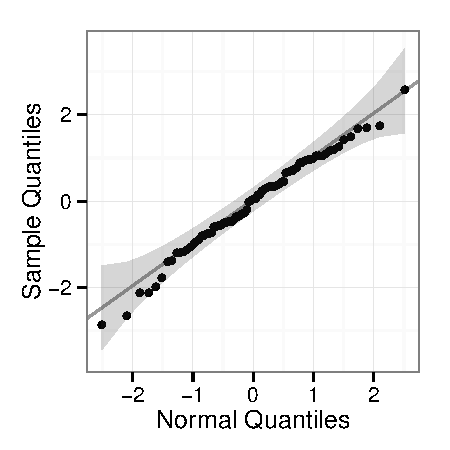
\includegraphics[width=0.33\linewidth]{lcr-intercept-qq.pdf}
		}
	  \subfloat[Random slopes]{
		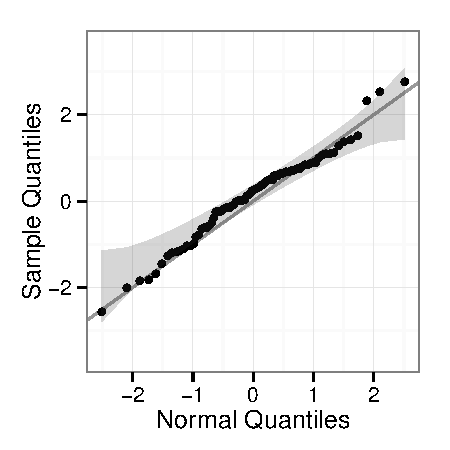
\includegraphics[width=0.33\linewidth]{lcr-slope-qq.pdf}
		}	
%	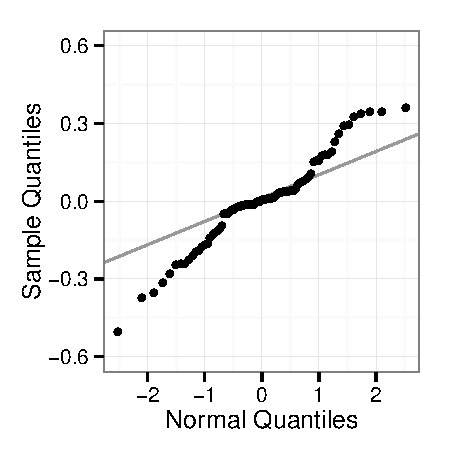
\includegraphics[width=0.32\textwidth]{raw-slope-qq.pdf}
	\caption{\label{fig:lcqq} Normal Q-Q plots of the minimally confounded random structures. The deviation from normality are much less pronounced than before -- in fact, it is questionable whether there is a significant amount of deviation; the results from the normal tests are not conclusive.}
\end{figure}

\begin{table}[ht]
\caption{\label{tab:edf2} Proportions of tests rejecting the null hypothesis of normality of the predicted error terms and random effects at the .05 significance level. 
}
\begin{center}
\begin{tabular}{l rrrr} \hline
 & \multicolumn{4}{c}{Test} \\  \cline{2-5}
 Residual & SW &  AD & CVM & KS \\ \hline
Error term			& 0.06 & 0.05 & 0.05 & 0.04 \\
Random intercept 	& \bf 0.04 & \bf 0.05 & \bf 0.05 & \bf 0.05 \\
Random slope 		& \bf 0.04 & \bf 0.04 & \bf 0.05 & \bf 0.05 \\
   \hline
\end{tabular}
\end{center}
\end{table}


\section{Exploring the Rotation Matrix}

The interpretation of minimally confounded residuals for purposes other than distributional assessment is complicated by the fact that they are linear combinations of residuals; however, the weights, $\bm{W}\trans$, are known, so interpretation is possible. Notice that the rows of $\bm{W}\trans$ give the weights specifying each linear combination and the columns give the weights assigned to each raw residual. Thus, the columns provide insight into the overall contribution of each raw residual and the rows of $\bm{W}\trans$ provide additional diagnostic information that, for example, can be used to investigate identified. In this section, each aspect will be investigated. To begin we explore the columns to better understand the rotation.

The average weights for each raw residual (column) show that residuals receiving larger weights are located in the center of the distribution of the raw residuals, while residuals receiving less weight are in the tails of the distribution. This is illustrated in Figure~\ref{fig:tailwts} for the predicted random effects using a linked histogram of average weights (right) and Q-Q plot of raw residuals (left).
%
\begin{figure}[htbp]
	\centering
	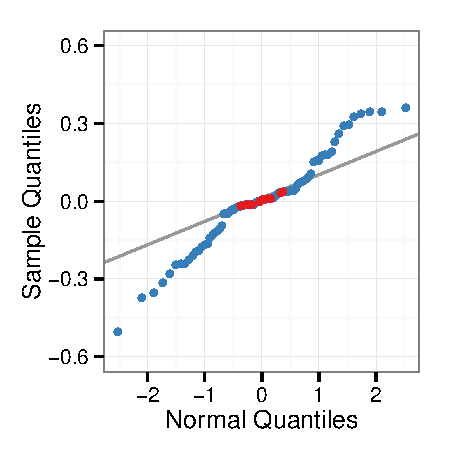
\includegraphics[width=0.4\linewidth]{qq-wts-tail.pdf}
	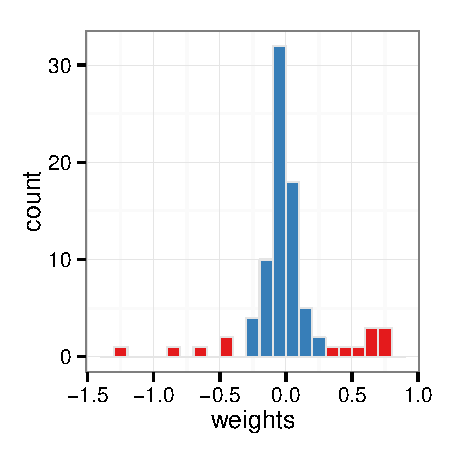
\includegraphics[width=0.4\linewidth]{hist-wts-tail.pdf}
	\caption{\label{fig:tailwts} Q-Q plot (left) and histogram (right) of the average weight for each raw residual given by $\bm{W}\trans$. The largest weights (red) correspond to residuals in the central region of the distribution of raw residuals.}
\end{figure}
%
To gain further insight, we must consider the entries of weight matrix.
%the two elements that comprise the rotation matrix: the relative precision factor of $\bm{B}$, $ \bm{\Lambda_r}^{-1/2} \bm{T_r}\trans$, and the orthogonal rotation matrix, $\bm{U}$.

%\begin{figure*}[htb]
%\centering
%	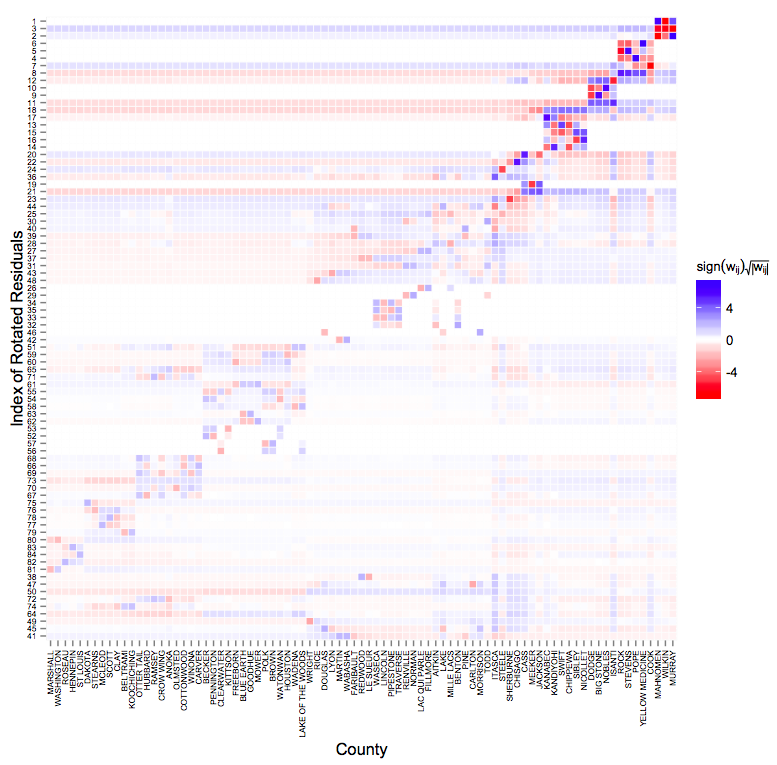
\includegraphics[width=0.9\textwidth]{tmslope-image.png}
%	\caption{\label{fig:matimage} Heat map of $\bm{W}\trans$ for the predicted random slopes ordered by the variance of the predicted random effects. The entries were transformed to improve interpretability.
%	}
%	
%\end{figure*}

Figure~\ref{fig:matimage} is a heat map of the  matrix of weights $\bm{W}$ for predicted random slopes  ordered by the variance of the predicted random slopes (with highest variance on the right).  Note that entries are scaled to their signed square root because of skewness in the weights. A block diagonal structure becomes apparent  in the heat map. This indicates  that terms with similar variances are treated similarly in the rotation to the least confounded direction. For example, Wilkin, Murray, and Mahnomen counties have the most variable predictions and are clustered together at the top right. Additionally, the horizontal lines that appear in the top portion of the heat map align with more confounded residuals, showing how information is combined to address this issue. Looking at the rows of the heat map will also aid in the interpretation of outlying points to determine whether a few observations are dominant or if many observations contribute equally.


%The relative precision factor of $\bm{B}$ performs the variance-covariance standardization of the residuals, and provides information about the relationships between residuals. Figure~\ref{fig:matimage} is a heat map of the relative precision factor for the variance of the predicted random slope that has been ordered by the variance of the predicted random slopes (with highest variance on the right). To aid interpretability, the entries were transformed into their signed square root. There is a clear block diagonal structure in this heat map that reveals counties with similar variances. For example, Wilkin, Murray, and Mahnomen counties have the most variable predictions and are clustered together at the top right. Additionally, the horizontal lines, which diminish from top right to bottom left, align with the amount of confounding in each predicted random slope. This matches expectations, since the confounding and pooling are interrelated, and estimates corresponding to highly confounded residuals will have a higher levels of pooling.

%For example, if an outlier is detected using the least confounded residuals, examination of the entries in the corresponding row of $\bm{M}\trans$ will reveal whether a few observations are dominant or if many contribute equally.



\section{Discussion}
We have shown that minimally confounded residuals are standardized, uncorrelated, homoscedastic residuals that address the concerns arising from the use of residuals for distributional assessment in the presence of pooling. The minimally confounded residuals can be used with Q-Q plots, which are familiar to analysts. While these residuals simplify the investigation of distributional assessment, they are linear combinations of residuals, and as such, are not directly applicable to the assessment of other aspects of the model, such as outlier detection; however, an investigation of the weights enables further investigation of unusual observations.
%
%however, investigation of the rotation matrix, $\bm{M}$, is itself of diagnostic interest.
%
%The rotation matrix, $\bm{M}$, is composed of the inverse square root matrix of the target residual, $ \bm{\Lambda_r}^{-1/2} \bm{T_r}\trans$,  and an orthogonal rotation matrix, $\bm{U}$. Both of these matrices are of diagnostic interest. Examination of the inverse square root matrix 
%
%\todo[inline]{I still need to figure out what to say about these matrices individually. I have been looking into them, and am still formulating what information they give us.}
%
It is important to note that goodness-of-fit tests are available for residuals at each level of the model \citep{Jiang:2001up}, but they do not lend themselves to graphical inspection, which is the focus of this paper, and the largely preferred method of distributional assessment. 

\end{document}